\documentclass[handout]{beamer}
%[handout]

\mode<presentation>
{
  \usetheme{Berkeley}
  \setbeamercovered{transparent}
  \setbeamertemplate{navigation symbols}{}
}

\usepackage[spanish]{babel}
\usepackage[utf8]{inputenc}
\usepackage{times}
\usepackage{tikz}
\usepackage{marvosym}

\usetikzlibrary{shapes,arrows,positioning}
\setbeamerfont{author}{size=\fontsize{10}{10}\bfseries}
\setbeamerfont{institute}{size=\fontsize{9}{12}\bfseries}
\setbeamerfont{title}{size=\fontsize{17}{18}\bfseries}
\setbeamerfont{subtitle}{size=\fontsize{12}{12}\bfseries}
\definecolor{darkblue}{RGB}{51,51,179}
\definecolor{darkgreen}{RGB}{0, 128, 0}
\newcommand\Fontable{\fontsize{9}{10}\selectfont}


\setbeamertemplate{title page}{

\begin{tikzpicture}[remember picture,overlay]

%\fill[darkblue]
%  ([yshift=15pt,xshift=-20pt]current page.west) rectangle (current page.north east);

\coordinate [below=2.5cm] (midpoint) at (current page.north);

\node [name = logo-iapso,
below= -0.4cm,
anchor = base,
%minimum width=\paperwidth,
%minimum height=1cm
inner sep=10pt] at (midpoint) {
\includegraphics[width=\paperwidth]{./imagenes/logo-iapso}};

\node [name=subtitle,
below = 0.2cm,
anchor=base,
%fill=darkblue,
text = white,
minimum width=\paperwidth,
minimum height=1cm] 
at (midpoint)  {\parbox[t]{\paperwidth}{\centering
 \usebeamerfont{subtitle}\textcolor{black}{%
    {\insertsubtitle}}}};

\node [name=title,
below = 1cm,
anchor=base,
fill=darkblue,
%text = white,
minimum width=\paperwidth,
minimum height=1cm] 
at (midpoint)  {\parbox[t]{0.9\paperwidth}{\centering
 \usebeamerfont{title}\textcolor{white}{%
    {\inserttitle}}}};

\node [name=author,
below = 3.2cm,
anchor=base,
%fill=darkblue,
text = white,
minimum width=\paperwidth,
minimum height=1cm] 
at (midpoint)  {\parbox[t]{\textwidth}{\centering
 \usebeamerfont{author}\textcolor{black}{%
    {\insertauthor}}}};
    
\node [name=institute,
below left = 4.2cm and 0.4cm,
anchor=base,
%fill=darkblue,
text = white,
minimum width=\paperwidth,
minimum height=1cm] 
at (midpoint)  {\parbox[t]{0.44\paperwidth}{\centering
 \usebeamerfont{institute}\textcolor{black}{%
    {\insertinstitute}}}};
    
\node [name = logo-armada,
below left = 6.5cm and 4.7cm,
anchor = base,
%minimum width=\paperwidth,
%minimum height=1cm
inner sep=10pt] at (midpoint) {
\includegraphics[width=0.2\paperwidth]{./imagenes/logo-arm}};

\node [name = logo-unidef,
below right = 5.5cm and 4.2cm,
anchor = base,
%minimum width=\paperwidth,
%minimum height=1cm
inner sep=10pt] at (midpoint) {
\includegraphics[width=0.27\paperwidth]{./imagenes/logo-unidef}};

\end{tikzpicture}
}

\author[Cinquini et al]{\textit{Mariano Cinquini, Patricio Bos, Igor Prario and Silvia Blanc}}
\institute[DIIV - UNIDEF]{Underwater Sound Division. 

Argentinian Navy Research Office. 

UNIDEF 

(National Council of Scientific and Technical Research / Ministry of Defense).}
\title[Advances on...]{Advances on modelling, simulation and signal processing of ultrasonic scattering responses from phytoplanktonic cultures}
\subtitle{}

\pgfdeclareimage[height=1.55cm]{symposium-logo}{./imagenes/logo-iugg.png}
\logo{\pgfuseimage{symposium-logo}}



% Delete this, if you do not want the table of contents to pop up at
% the beginning of each subsection:
%\AtBeginSection[]
%{
%  \begin{frame}<beamer>{}
%  	\vspace{3px}
%    \tableofcontents[currentsection,currentsubsection]
%  \end{frame}
%}
%
%\AtBeginSubsection[]
%{
%  \begin{frame}<beamer>{}
%	\vspace{3px}
%     \tableofcontents[currentsection,currentsubsection]
%  \end{frame}
%}

% If you wish to uncover everything in a step-wise fashion, uncomment
% the following command: 

\beamerdefaultoverlayspecification{<+->}


\begin{document}

\begin{frame}[plain,noframenumbering]
  \titlepage
\end{frame}

\section{Objectives and Introduction}

\begin{frame}{OBJECTIVES AND INTRODUCTION}
	\Fontable
	
		\begin{minipage}[c]{1\linewidth}
		\begin{minipage}[c]{0.6\linewidth}
			\begin{itemize}
				\item[]
				\item Development of noninvasive acoustic techniques, based on the volume backscattering phenomena for phytoplankton abundance estimation and further Harmful Algae Blooms \textbf{real-time} detection.
			\end{itemize}
		\end{minipage}
		\hspace{1px}
		\begin{minipage}[c]{0.38\linewidth}
			\visible<2-> {\centering 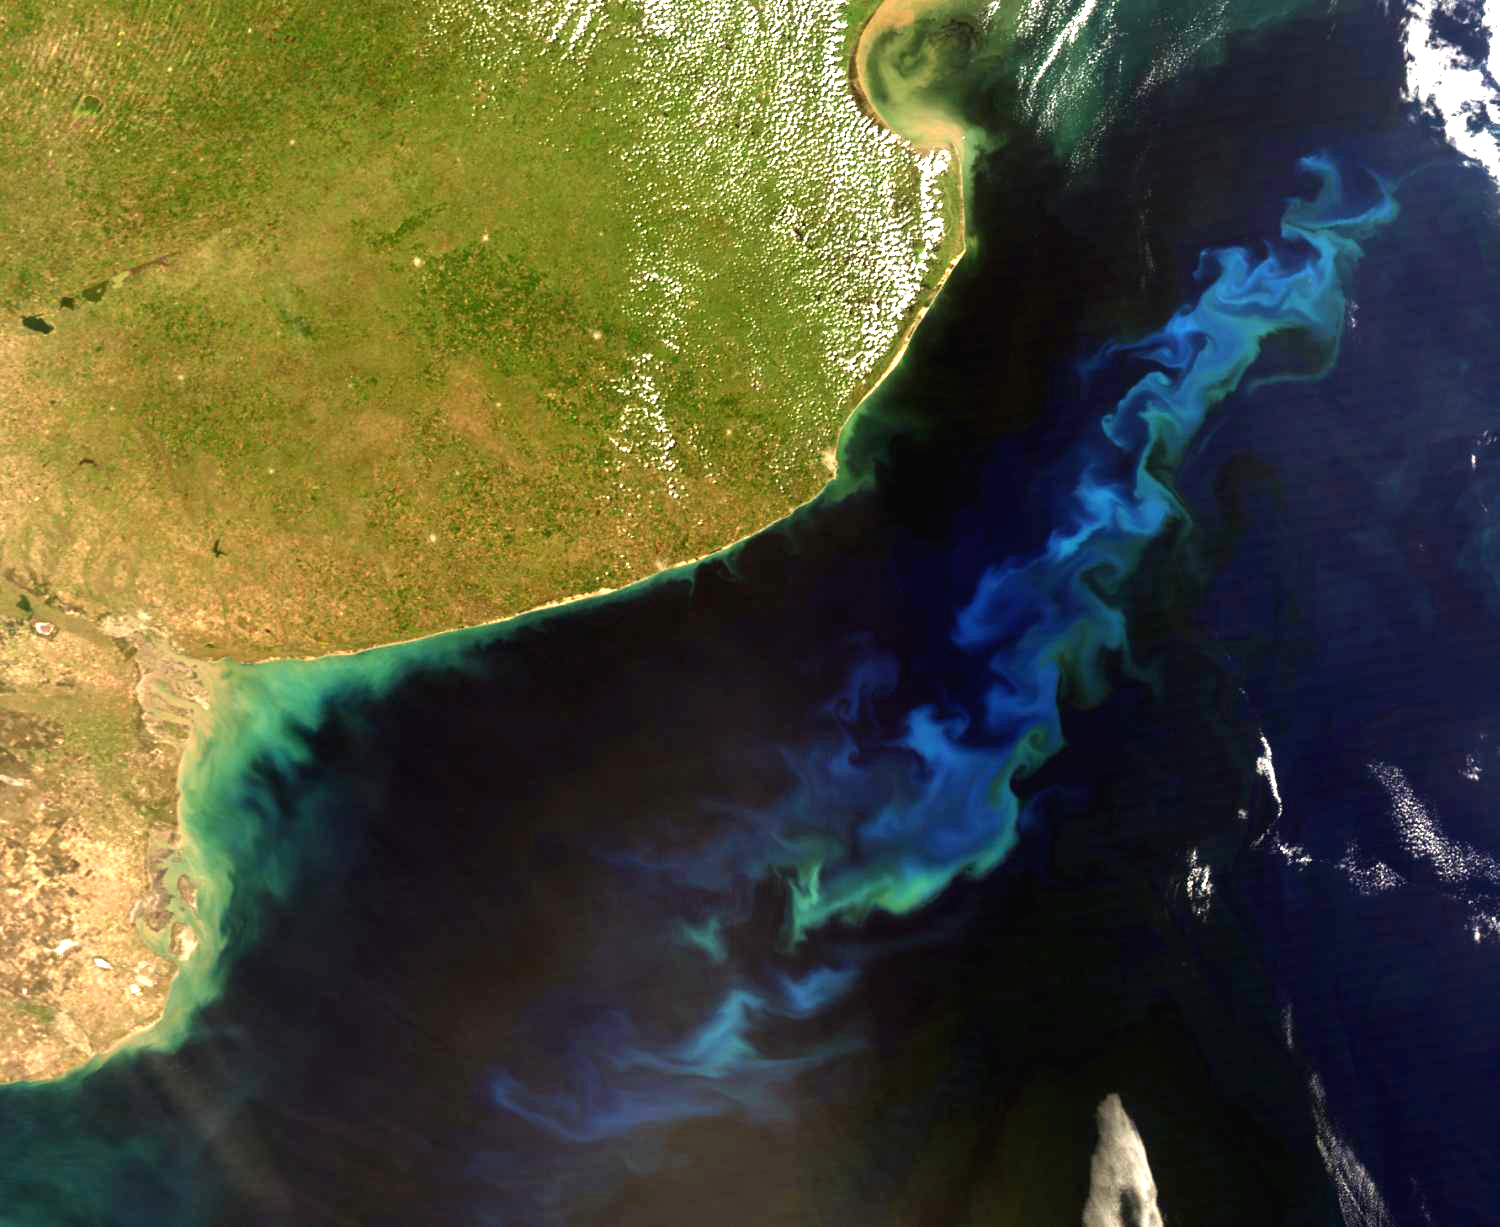
\includegraphics[width=0.24\paperwidth]{./imagenes/HAB1_brillante.jpg}}
		\end{minipage}
		\end{minipage}
	
		\vspace{2px}
		\begin{minipage}[c]{1\linewidth}
		\begin{minipage}[c]{0.45\linewidth}
			\begin{itemize}
				\item \textcolor{magenta}{Superar/mejorar los obstáculos vinculados al reducido tamaño de los dispersores, el bajo contraste de impedancias, y la limitada capacidad de discriminación de algas frente a dispersores espurios}
			\end{itemize}
		\end{minipage}
		\hspace{1px}
		\begin{minipage}[c]{0.53\linewidth}
			\visible<3-> {\centering 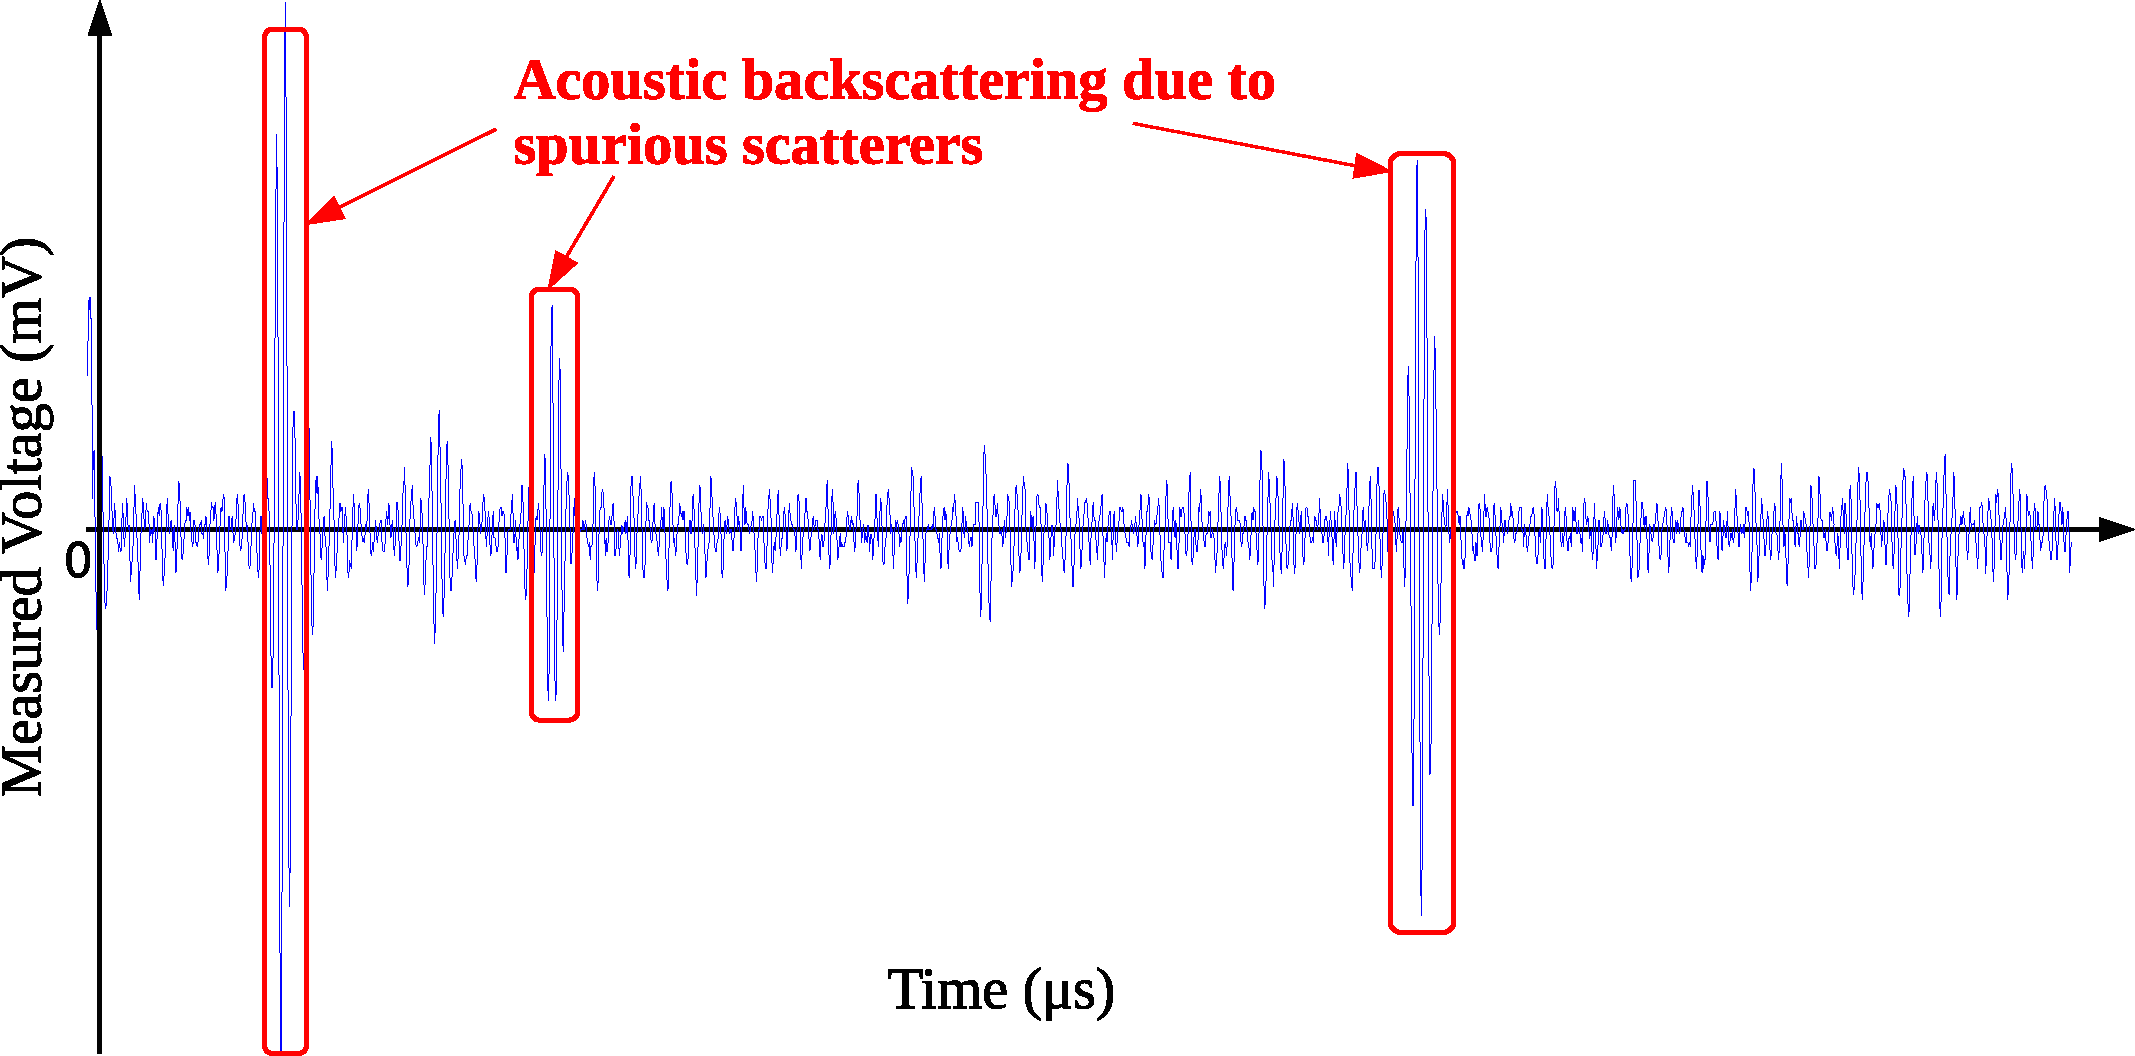
\includegraphics[width=0.4\paperwidth]{./imagenes/respuestones}}
		\end{minipage}
		
		\vspace{2px}
%				
		\end{minipage}
		
		\begin{itemize}		
		\item Validation of models and simulations employed in this work and optimization of the inteprepation of the at-lab measurementes carried out with the available equipment.
		\end{itemize}
		
\end{frame}

\section{Materials and Methods}

\subsection{Phytoplanktonic cultures}

\begin{frame}{MATERIALS AND METHODS - Phytoplanktonic cultures}
\Fontable

Phyoplanktonic single-species cultures of \textit{Skeletonema pseudocostatum} generated in the laboratory for insonification with ultrasonic equipment.

\begin{minipage}[c]{1\linewidth}
\begin{minipage}[c]{0.7\linewidth}
\begin{itemize}
	\Fontable
	\item<3-> Chain-forming cells shelled with silicon dioxide (increased Scattering Strengh, $S_v$)
\end{itemize}
\end{minipage}
\begin{minipage}[c]{0.29\linewidth}
\visible<2->{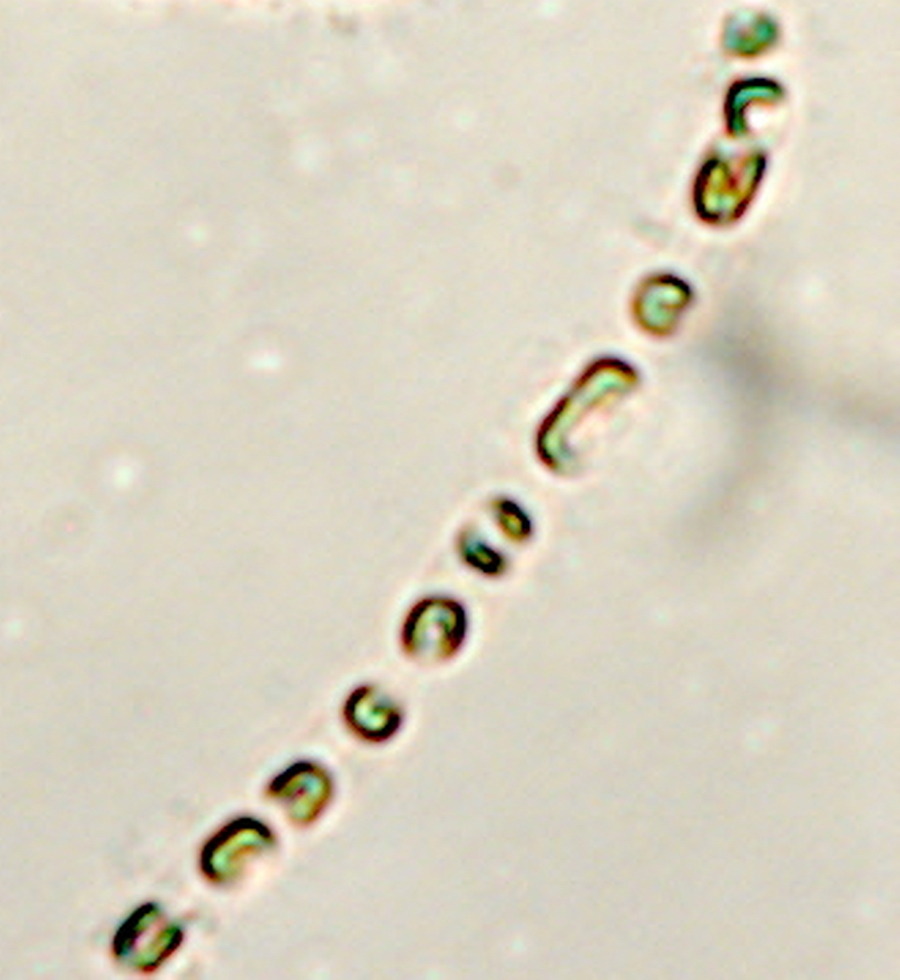
\includegraphics[width=0.17\paperwidth]{imagenes/skeleto_detalle_cadena.jpg}}
\end{minipage}
\end{minipage}

\begin{minipage}[c]{1\linewidth}
\begin{minipage}[c]{0.7\linewidth}
\begin{itemize}
	\Fontable
	\item<3-> Characteristic sizes of invidual and chained cells in the \textit{Rayleigh region}
\end{itemize}
\end{minipage}
\begin{minipage}[c]{0.29\linewidth}
\visible<2->{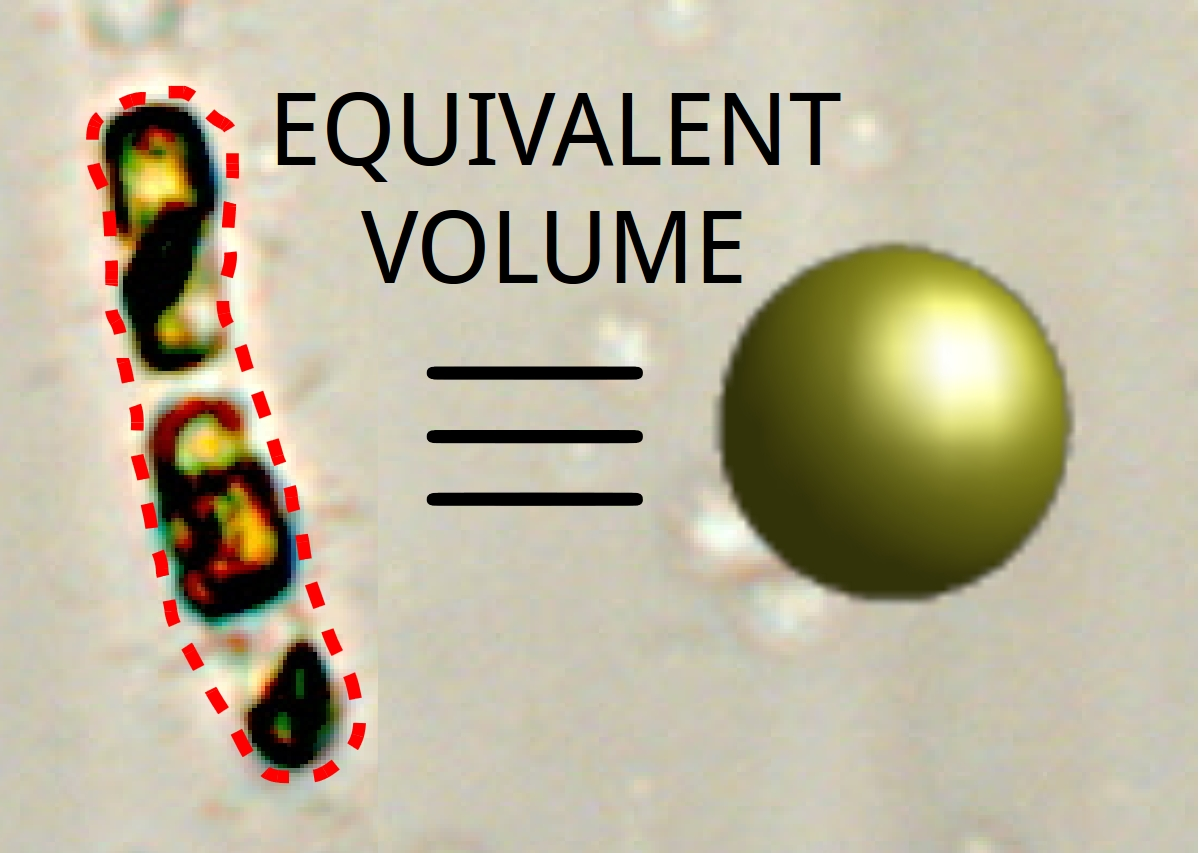
\includegraphics[width=0.22\paperwidth]{imagenes/equiv_volume.jpg}}
\end{minipage}
\end{minipage}

\begin{minipage}[c]{1\linewidth}
\begin{minipage}[c]{0.7\linewidth}
\begin{itemize}
	\Fontable
	\item<3-> Easy generation and maintenance in the laboratory
\end{itemize}
\end{minipage}
\begin{minipage}[c]{0.29\linewidth}
\visible<2->{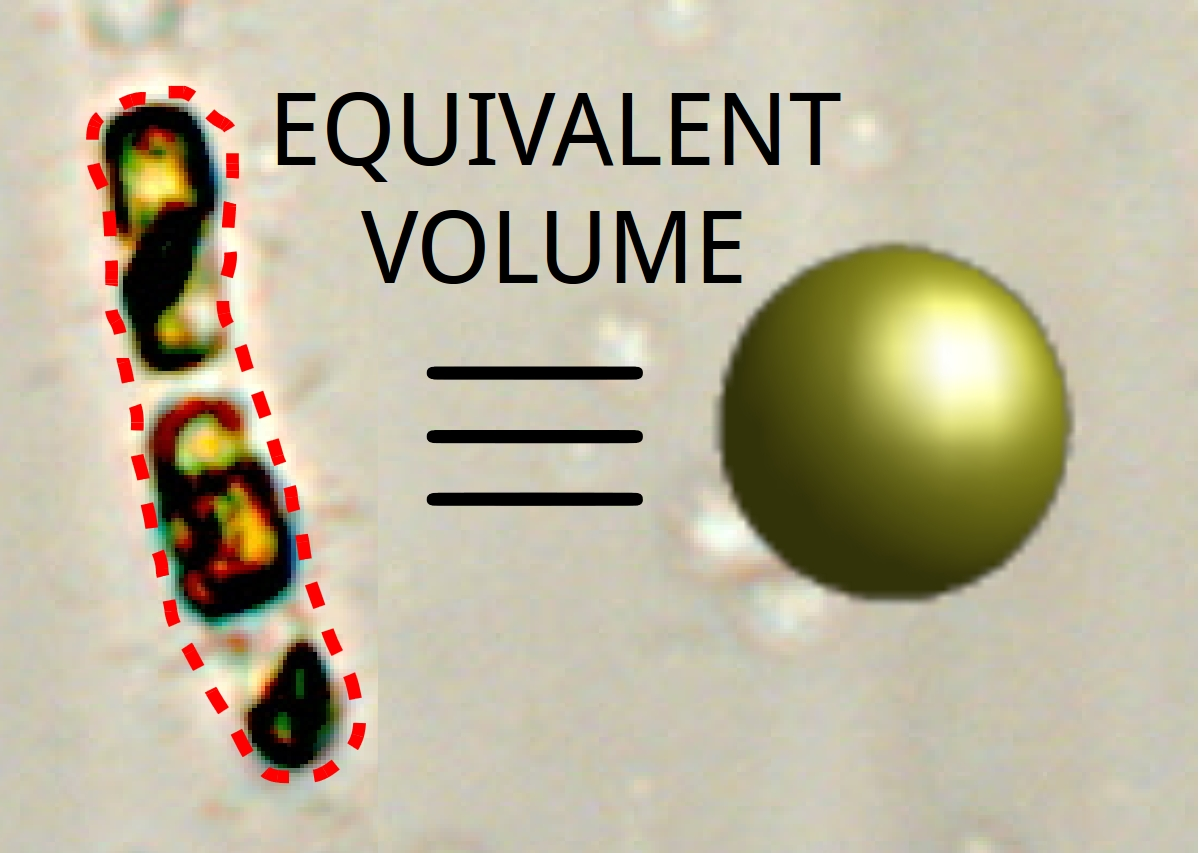
\includegraphics[width=0.22\paperwidth]{imagenes/equiv_volume.jpg}}
\end{minipage}
\end{minipage}

%		\item<3-> Easy\textcolor{magenta}{¿palabra más adecuada?} generation and maintenance in the laboratory
%		\item<3-> Bloom-forming species, being representative of the problem of HAB detection


\end{frame}


\begin{frame}{INTRODUCTION - Fundamentals of Volume Scattering Phenomena}
\Fontable
\begin{itemize}
\item<2-> When assumptions apply, $S_V$ depends on:
	\begin{itemize}
	\Fontable
		\item<2-> \textbf{Frequency}, $f$.
		\item<2-> Numerical Abundance, $N$.
		\item<2-> Relation between the wavelength, $\lambda$ and scatterers' characteristic size, $a$.
		\item<2-> \textbf{Density} and \textbf{sound speed contrasts} relative to the aqueous medium.
	\end{itemize}
	
\vspace{2mm}
\item<3-> For \textit{Rayleigh region} ($k  a \ll 1$, where $k=2\pi / \lambda)$, the scattered field is \textbf{isotropic}. Then,
\end{itemize}
\visible<3->{\[
\boxed{S_v = 10 \log \left( \frac{\sigma_v}{4\pi} \right)}
\]}
\visible<3->{where $\sigma_v$ (m$^{-1}$) is the {\textbf{Volume Backscattering Coefficient}}.}

\end{frame}

\begin{frame}{INTRODUCTION - Fundamentals of Volume Scattering Phenomena}
\Fontable
\begin{minipage}[c]{1\linewidth}
\begin{minipage}[c]{0.7\linewidth}
\begin{itemize}
\item[]
\item<2-> If there is a \textbf{dominant} type of scatterers with \textbf{low variability} size distribution, then
\visible<3->{\[ \boxed{ \sigma_v = N \sigma_{bs}} \]}
\visible<3->{where $\sigma_{bs}$ (m$^2$) is the average {\textbf{Backscattering Cross-Section}} of the individual scatterers.}
\vspace{1pc}
\item<4-> If there are several types of scatterers grouped by size,
\visible<5->{\[ \boxed{\sigma_v = \sum N_i {\sigma_{bs}}_i} \]}
\visible<5->{where $ N_i $ is the Numerical Abundance of the scatterers' $ith$-group  and $ {\sigma_{bs}}_i $ is the \textbf{corresponding Backscattering Cross-Section}.}
\end{itemize}
\end{minipage}
\begin{minipage}[c]{0.28\linewidth}

\tiny
\visible<2->{\textit{Chlamydomonas reinhardtii}} \\
\visible<2->{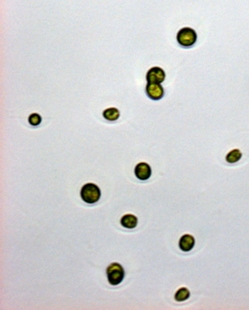
\includegraphics[width=0.2\paperwidth]{imagenes/clamis.jpg}}

\vspace{3mm}

\visible<4->{\textit{Skeletonema pseudocostatum}} \\
\visible<4->{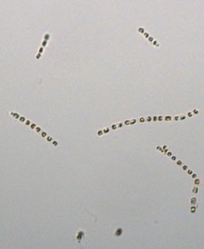
\includegraphics[width=0.2\paperwidth]{imagenes/skeletonema.jpg}}
\end{minipage}
\end{minipage}

\end{frame}

\section{Modelling}


\begin{frame}{MODELLING}
\Fontable
\visible<2->{Backscattering cross-section of \textcolor{darkgreen}{{\bf \textit{Skeletonema pseudocostatum}}} was estimated by three different approaches:}

\begin{minipage}[c]{1\linewidth}
\begin{minipage}[c]{0.6\linewidth}


\begin{enumerate}
\item<3-> \textbf{Johnson Modified model} (Blanc \textit{et al}, 2000): every individual scatterer is represented by an equivalent volume sphere.

\vspace{1cm}
\item<4-> \textbf{``Chain'' model} (Bok \textit{et al}, 2010): every chain of scatterers is represented by an equivalent volume sphere

\vspace{1.2cm}
\item<5-> \textbf{Prolate Spheroidal model} (González \textit{et al}, 2011, and Prario \textit{et al}, 2015): every chain of scatterers is represented by an equivalent volume prolate shperoid.
\end{enumerate}

\end{minipage}
\begin{minipage}[c]{0.36\linewidth}
\visible<3->{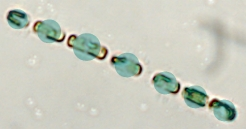
\includegraphics[width=0.28\paperwidth]{imagenes/johnson.jpg}}
\visible<4->{\centering{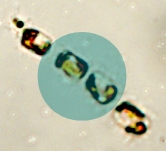
\includegraphics[width=0.22\paperwidth]{imagenes/cadenas.jpg}}}
\visible<5->{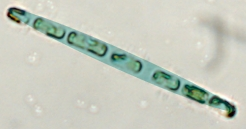
\includegraphics[width=0.28\paperwidth]{imagenes/prolado.jpg}}
\end{minipage}
\end{minipage}

\end{frame}

\section{Materials and Methods}
\subsection{Experimental Setup}

\begin{frame}{MATERIALS AND METHODS - Experimental setup}
\Fontable
\begin{itemize}
\item []
\item<2-> Insonification of \textcolor{darkgreen}{{\bf \textit{Skeletonema pseudocostatum, Euglena gracilis}}} and \textcolor{darkgreen}{{\bf \textit{Chlamydomonas reinhardtii}}} liquid cultures with 2.25, 3.5 and 5 MHz ultrasonic transducers by pulsed excitation.
\item<3-> Signal conditioning and amplification.
\item<4-> Acquisition and processing.
\end{itemize}


\raisebox{5mm}{\visible<	
2->{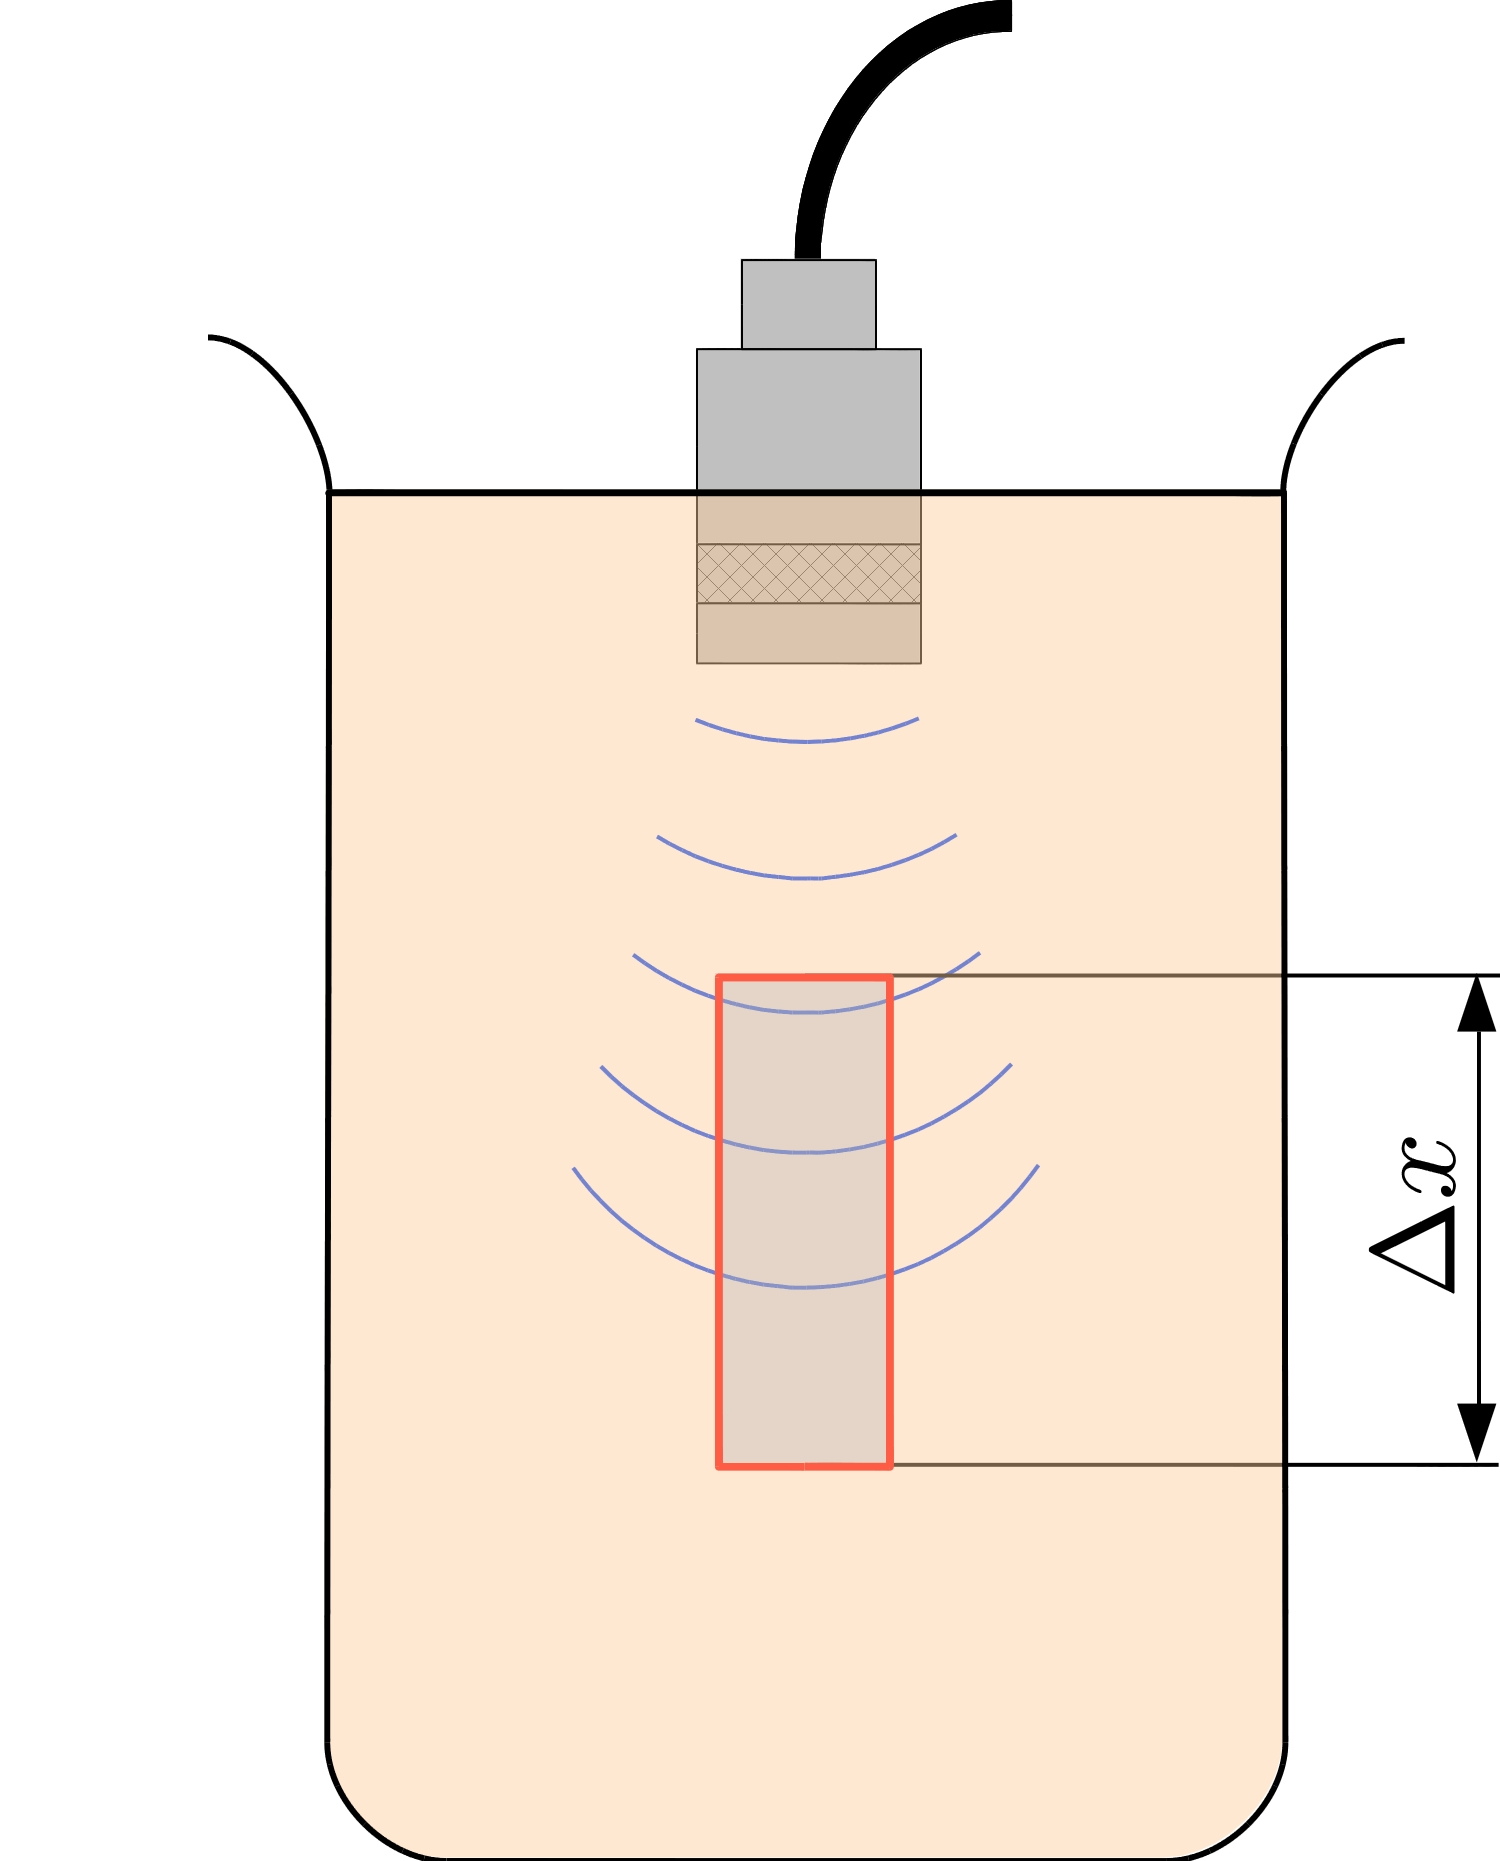
\includegraphics[width=0.22\paperwidth]{imagenes/vaso.jpg}}}
\only<1>{
\includegraphics[width=0.55\paperwidth]{imagenes/white2.jpg}}
\only<2>{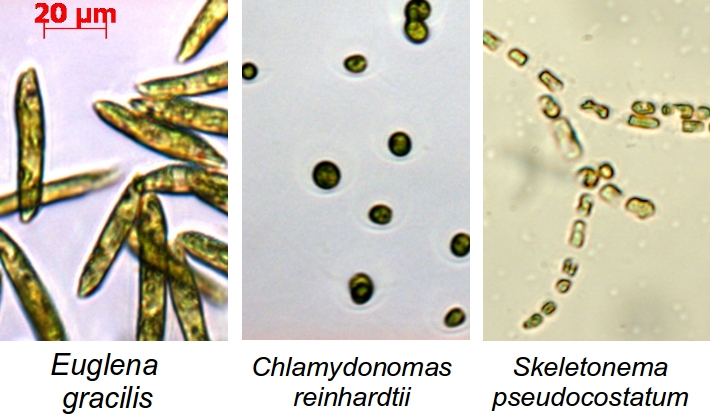
\includegraphics[width=0.55\paperwidth]{imagenes/especies.jpg}}
\only<3>{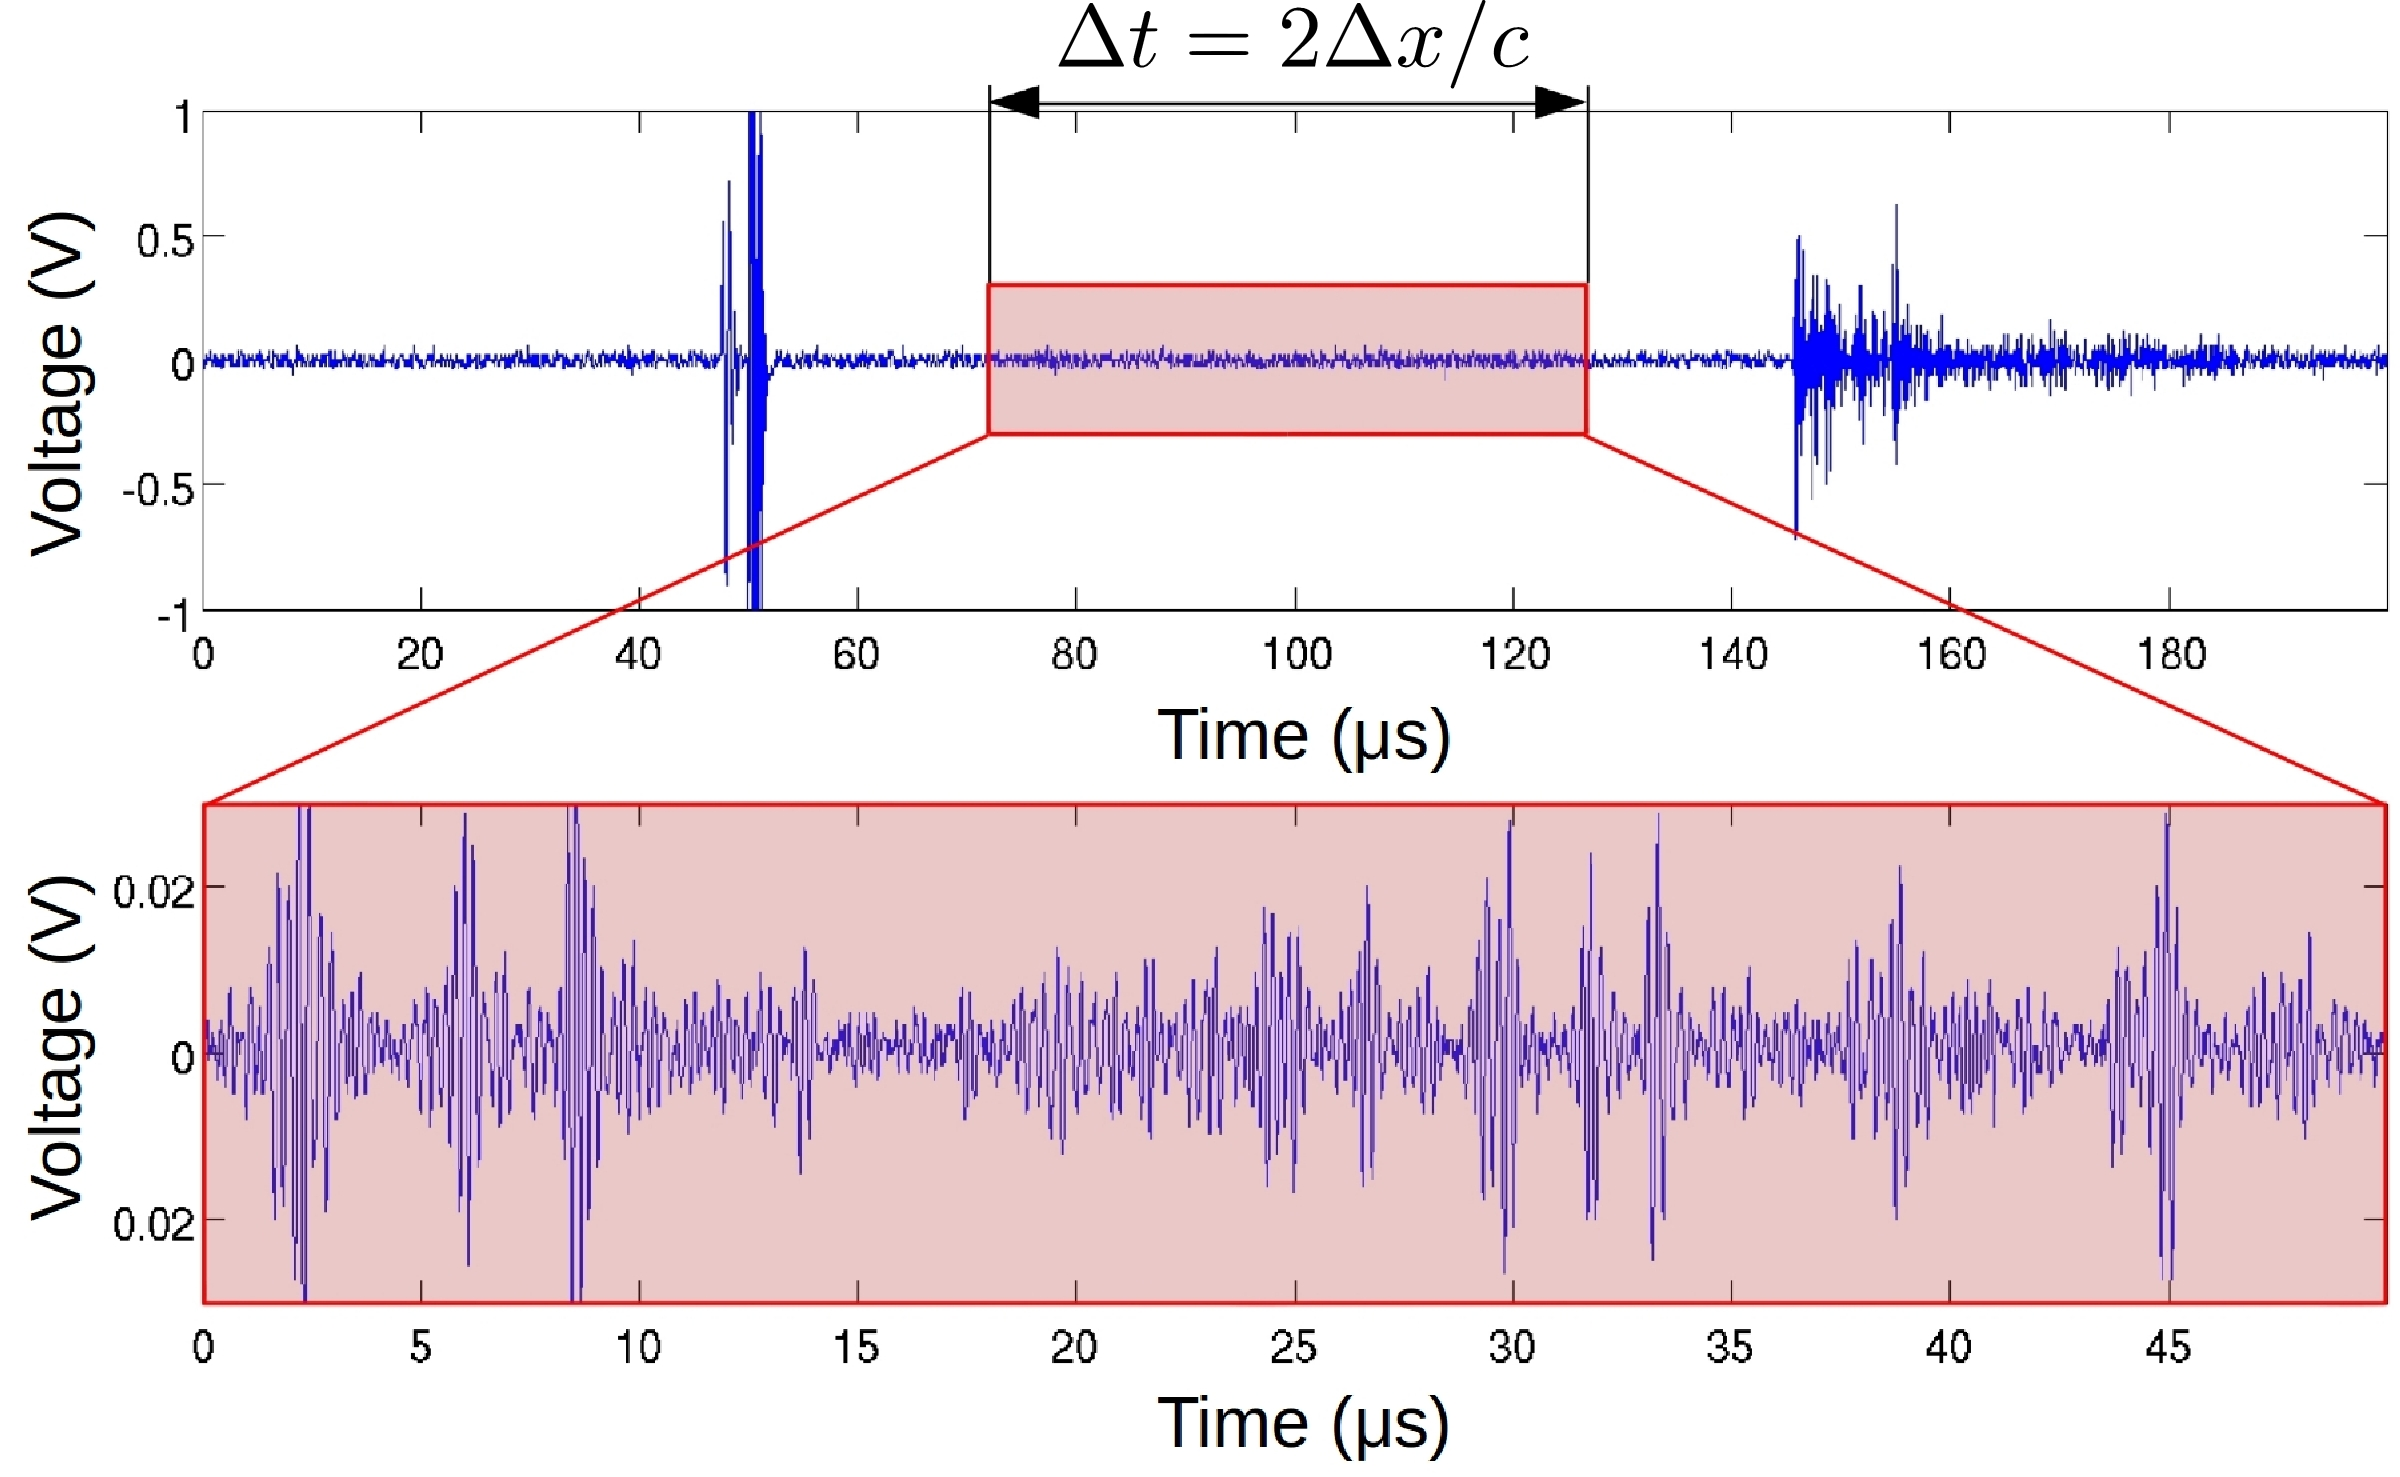
\includegraphics[width=0.55\paperwidth]{imagenes/pulso-eco_y_detalle3_ingles2.jpg}}
\only<4->{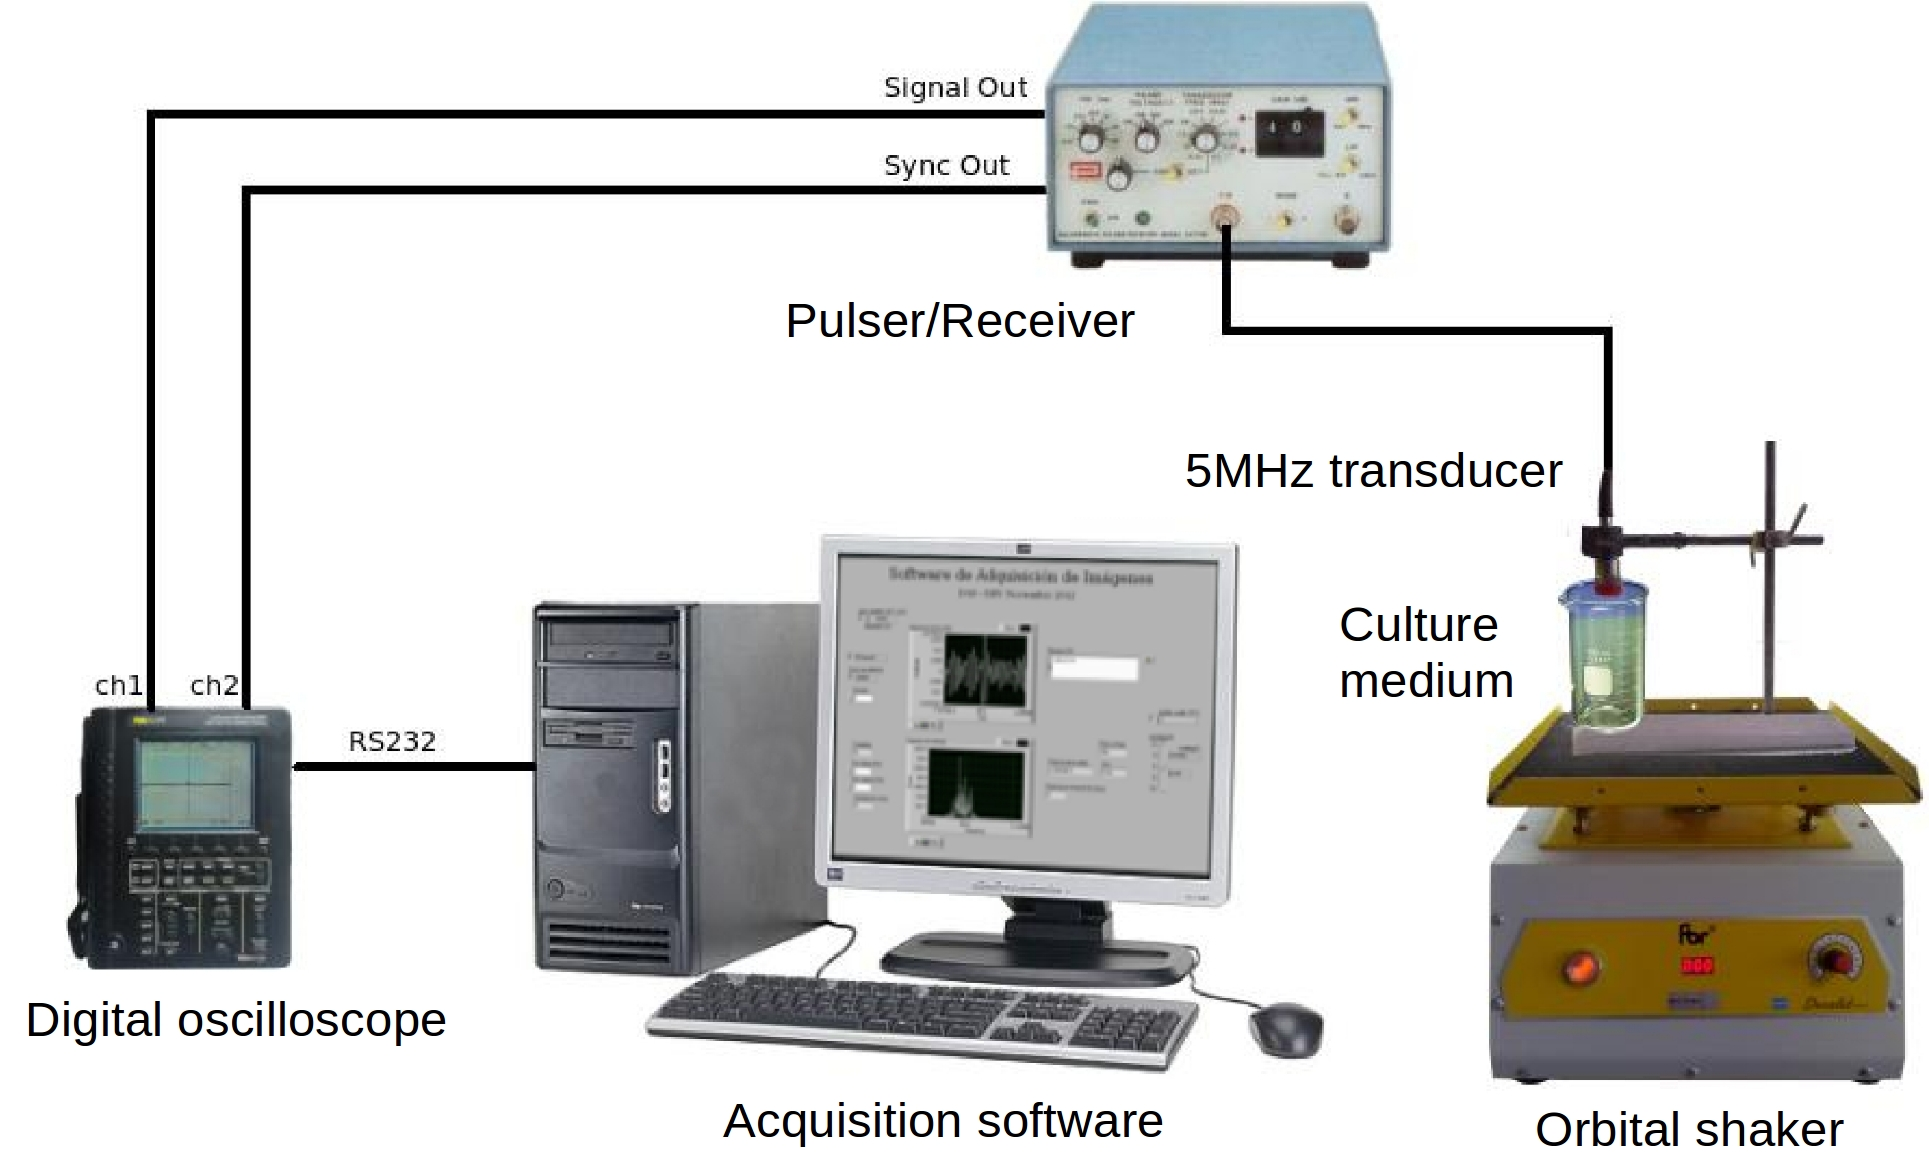
\includegraphics[width=0.55\paperwidth]{imagenes/banco_medicion_ingles.jpg}}

\end{frame}

\subsection{Minimization of Spourious scatterers effect}

\begin{frame}{MATERIALS AND METHODS - Minimization of spurious scatterers effect}
\Fontable
\begin{itemize}
\item<2-> The existence of undesired scatterers along the insonified volume (bubbles and suspended particles) \textbf{affects} the total backscattered power.

\vspace{2px}
\centering
\only<1-2>{
\includegraphics[width=0.64\paperwidth]{imagenes/white.jpg}}
\only<3-4>{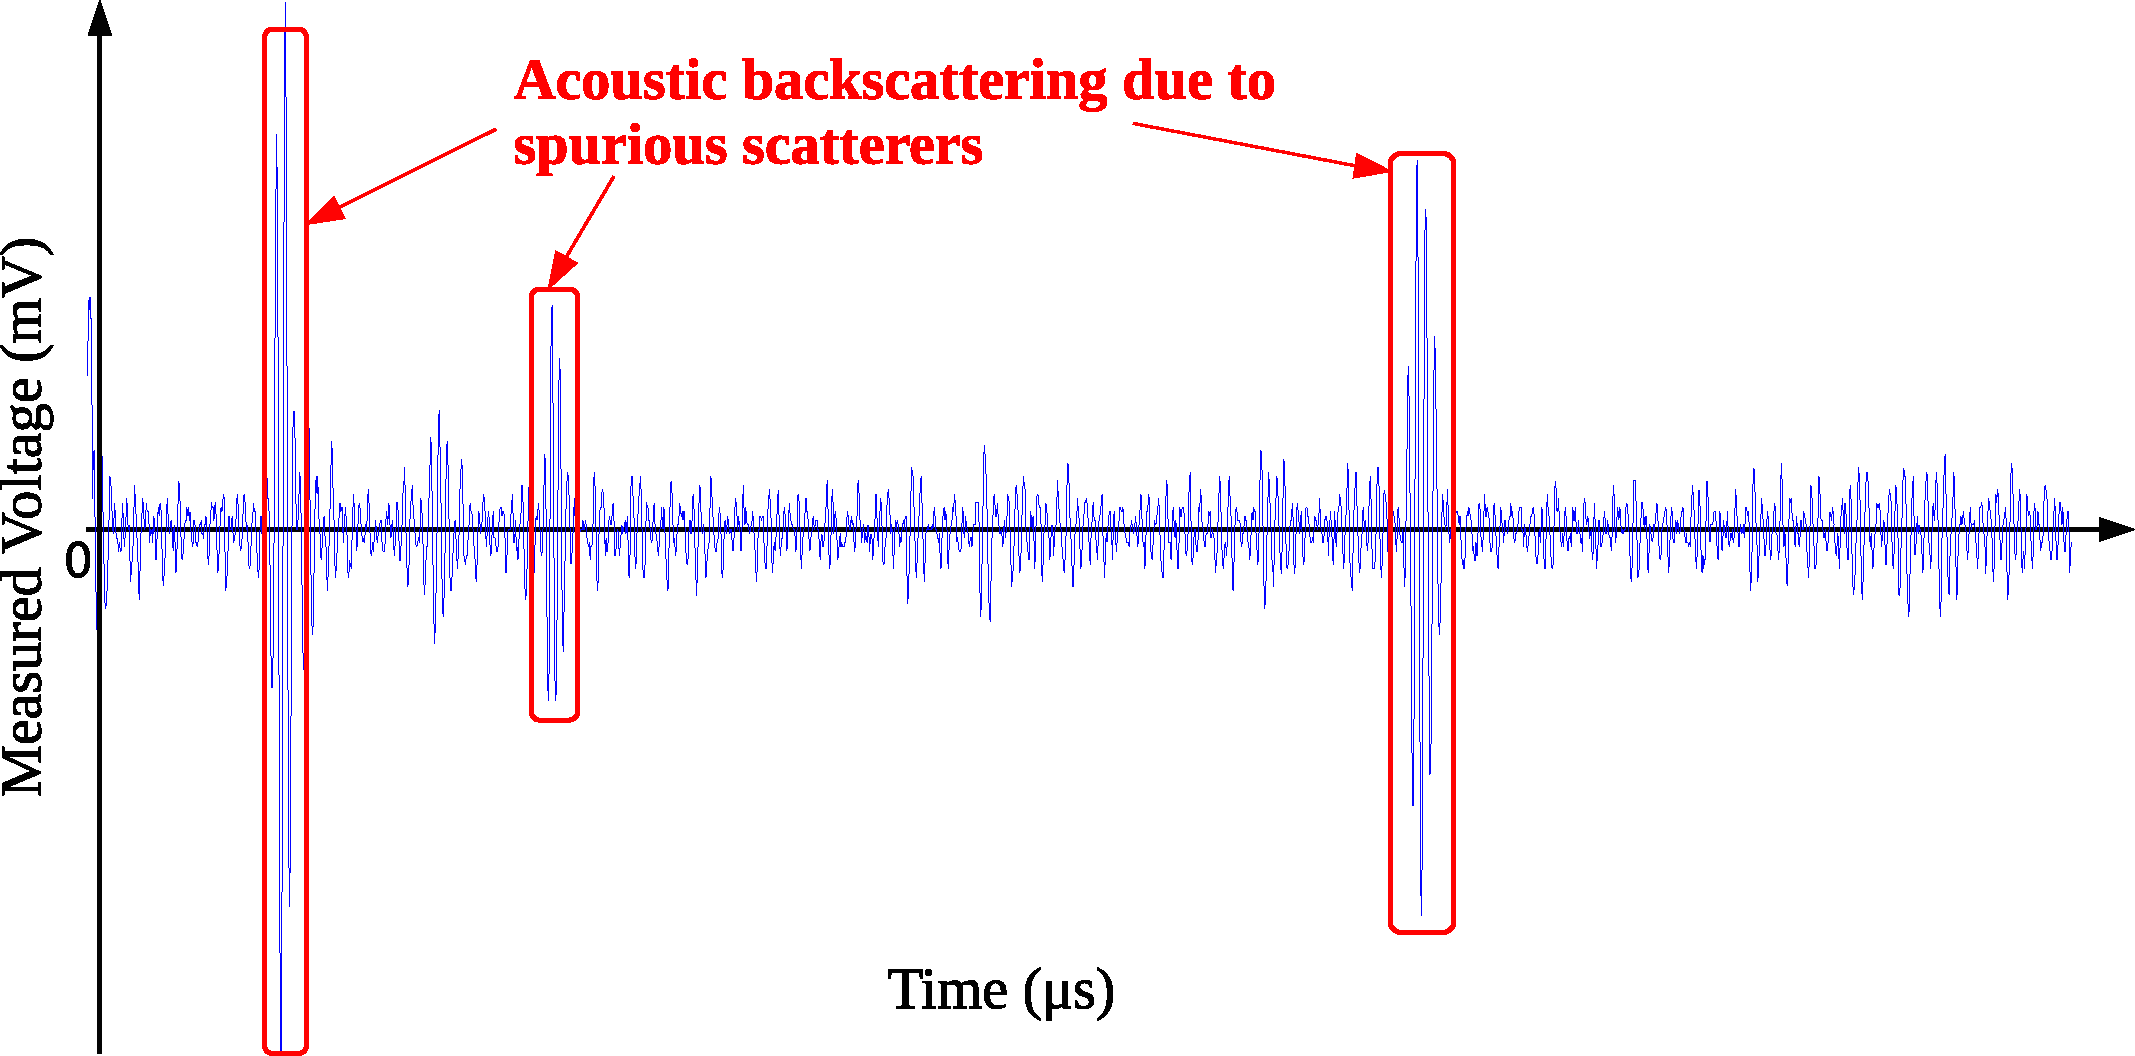
\includegraphics[width=0.67\paperwidth]{imagenes/respuestones.pdf}}
\only<5->{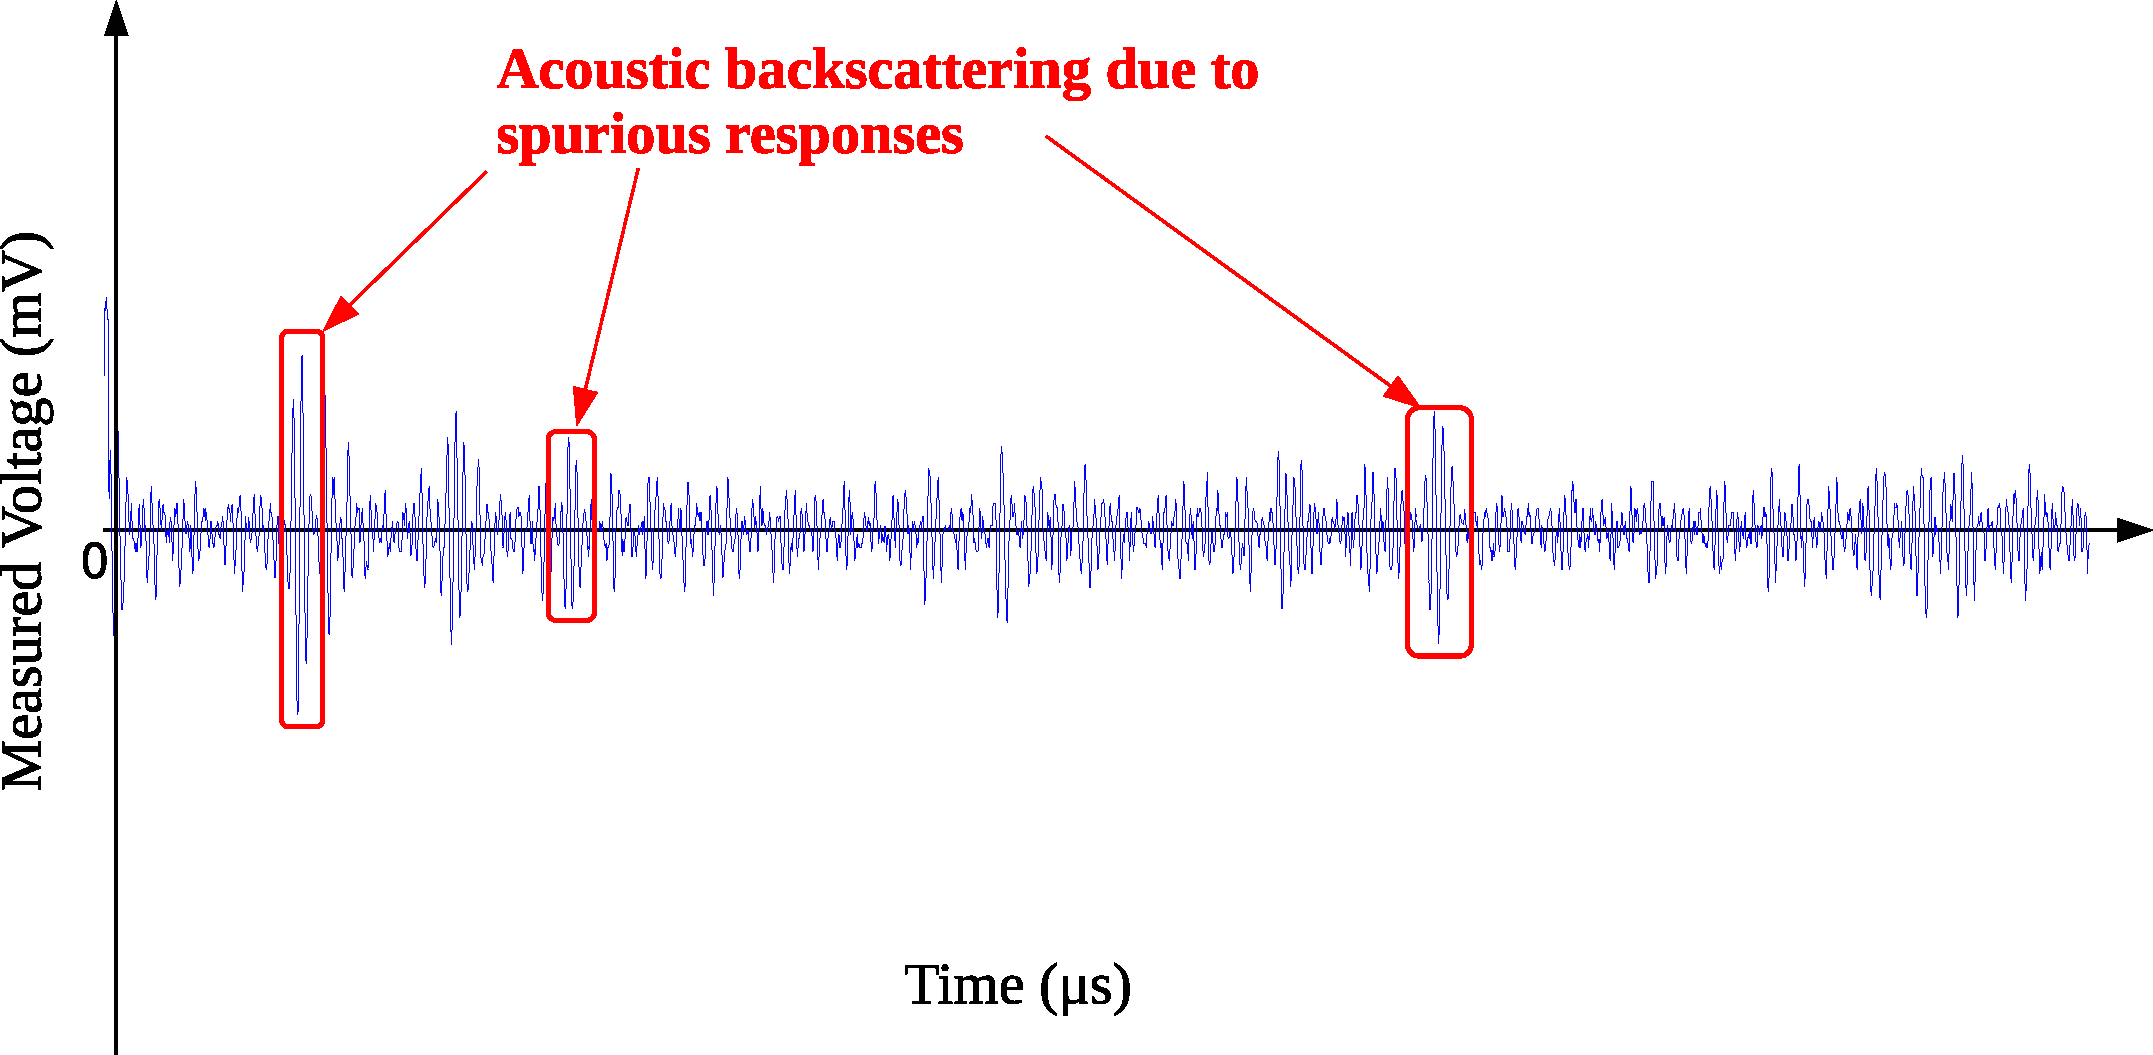
\includegraphics[width=0.67\paperwidth]{imagenes/respuestones2.pdf}}
\end{itemize}

\vspace{3px}
\visible<4-> {\bf When the spurious acoustic responses amplitudes and shapes are \textit{not} easily detectable,} 
\visible<6->{\textcolor{darkblue}{\bf \textit{signal processing techniques} should be applied}.}

\end{frame}

\begin{frame}{MATERIALS AND METHODS - Minimization of spurious scatterers effect}
\Fontable
\begin{minipage}[c]{1\linewidth}
\begin{minipage}[c]{0.46\linewidth}
\begin{itemize}
\item<2-> Acquisition of ensembles of $\sim 300$ backscattered signals. 
\item<2-> Segmentation of each signal in intervals of $\sim 1\hspace{1px}\mu s$.

\vspace{2pc}
\item<3-> Narrowband filtering (centered at the transducer frequency) and signal power computation for \textbf{each} segment.
\item<3-> Computation of filtered to non-filtered signal power ratio for \textbf{each} segment.
\item<4-> Two-dimensional histogram representation.
\end{itemize}

\end{minipage}
\begin{minipage}[c]{0.55\linewidth}
\visible<2->{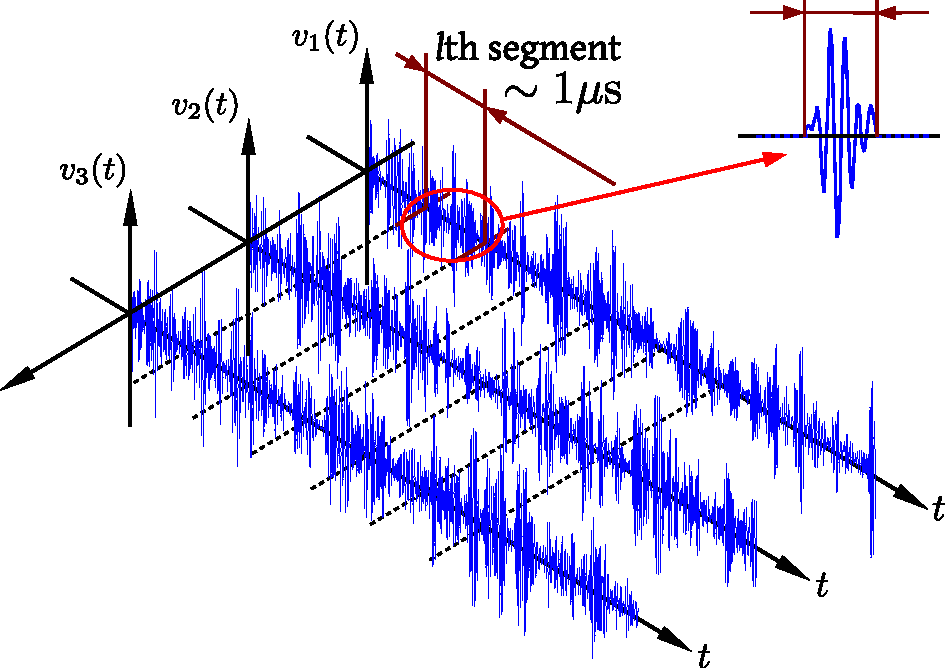
\includegraphics[width=0.41\paperwidth]{imagenes/segmentacion1.pdf}}

\hspace{1pc}\visible<4->{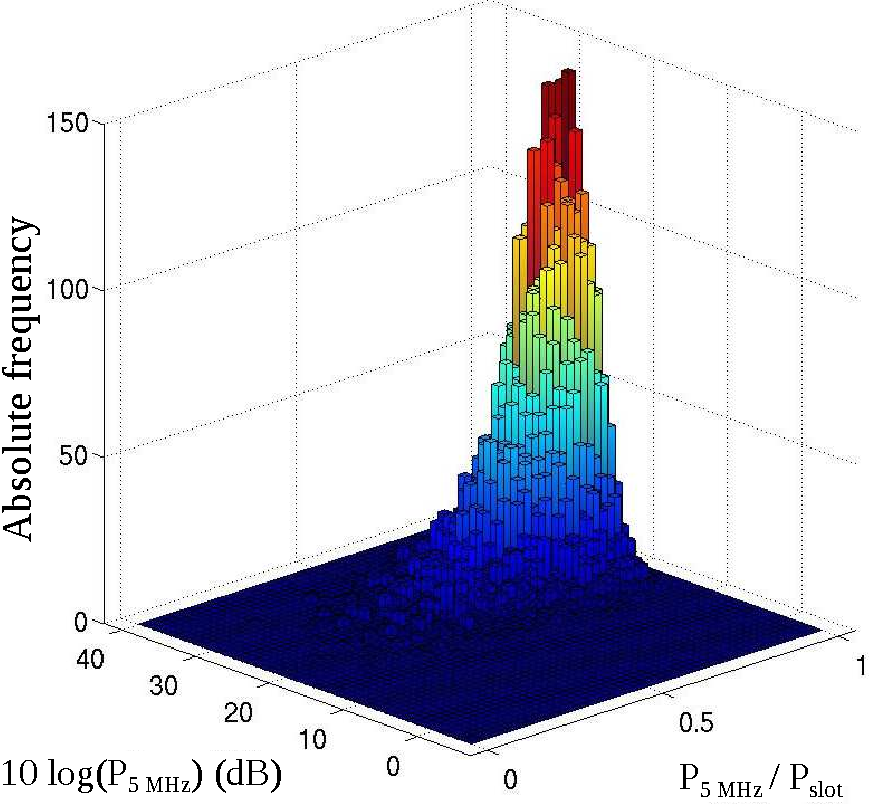
\includegraphics[width=0.33\paperwidth]{imagenes/hist3d_ok.pdf}}
\end{minipage}
\end{minipage}


\end{frame}

\subsection{$S_v$ determination}

\begin{frame}{MATERIALS AND METHODS - Determination of Volume Backscattering Strength, $S_v$}
\Fontable
\begin{minipage}[c]{1\linewidth}
\begin{minipage}[c]{0.46\linewidth}
\begin{itemize}
\vspace{1pc}
\item<2-> Mean signal power was computed by averaging the power of the bins with frequencies above a selected threshold.
\item<3-> From the experimental viewpoint, non-dependent on any model, the Volume Backscattering Strength, $S_v$, can be expressed as
\item<4-> Identical transducers were used to measure the incident and backscattered intensities. This fact enabled to calculate $S_v$ without taking into account any sensitivity values.
\end{itemize}
 
\end{minipage}
\begin{minipage}[c]{0.55\linewidth}
\visible<2->{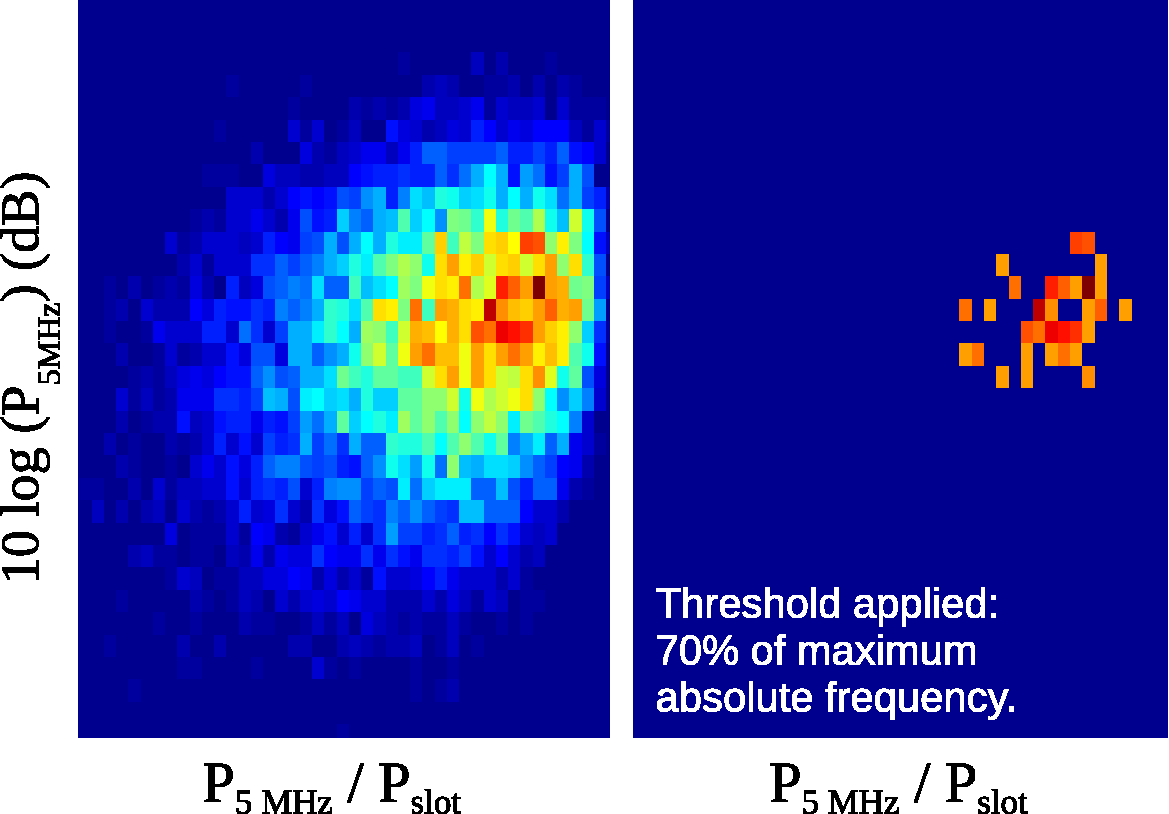
\includegraphics[width=0.41\paperwidth]{imagenes/umbral_ok2.pdf}}


\hspace{1pc}\visible<3->{
\[
\textcolor{darkblue}{\boxed{S_v = 10 \log \left( \frac{ \langle v_{bs}^2 \hspace{1px} \rangle 2}{v_{inc}^2 \hspace{1px} c \tau \psi} \right)}}
\]
}
\scriptsize

\visible<3->{
\hspace{2pc}where

\hspace{2pc}$\langle v_{bs}^2 \rangle \propto$ backscattered intensity

\hspace{2pc}$v_{inc}^2 \propto$ incident intensity

\hspace{2pc}$c \;\rightarrow$  sound speed in the medium

\hspace{2pc}$\tau \;\rightarrow$ pulse duration

\hspace{2pc}$\psi \;\rightarrow$ equivalent beam width
}


\end{minipage}
\end{minipage}

\end{frame}

\section{RESULTS}
\subsection{Detection of backscattering phenomena}

\begin{frame}{RESULTS - Detection of backscattering phenomena}
\Fontable
\visible<2->{Computation of backscattered power ratios for culture media {\bf \textit{with} and \textit{without}} phytoplankton, for the three species at three frequencies.}

\vspace{1pc}
\centering
\visible<2->{\hspace{-2pc} 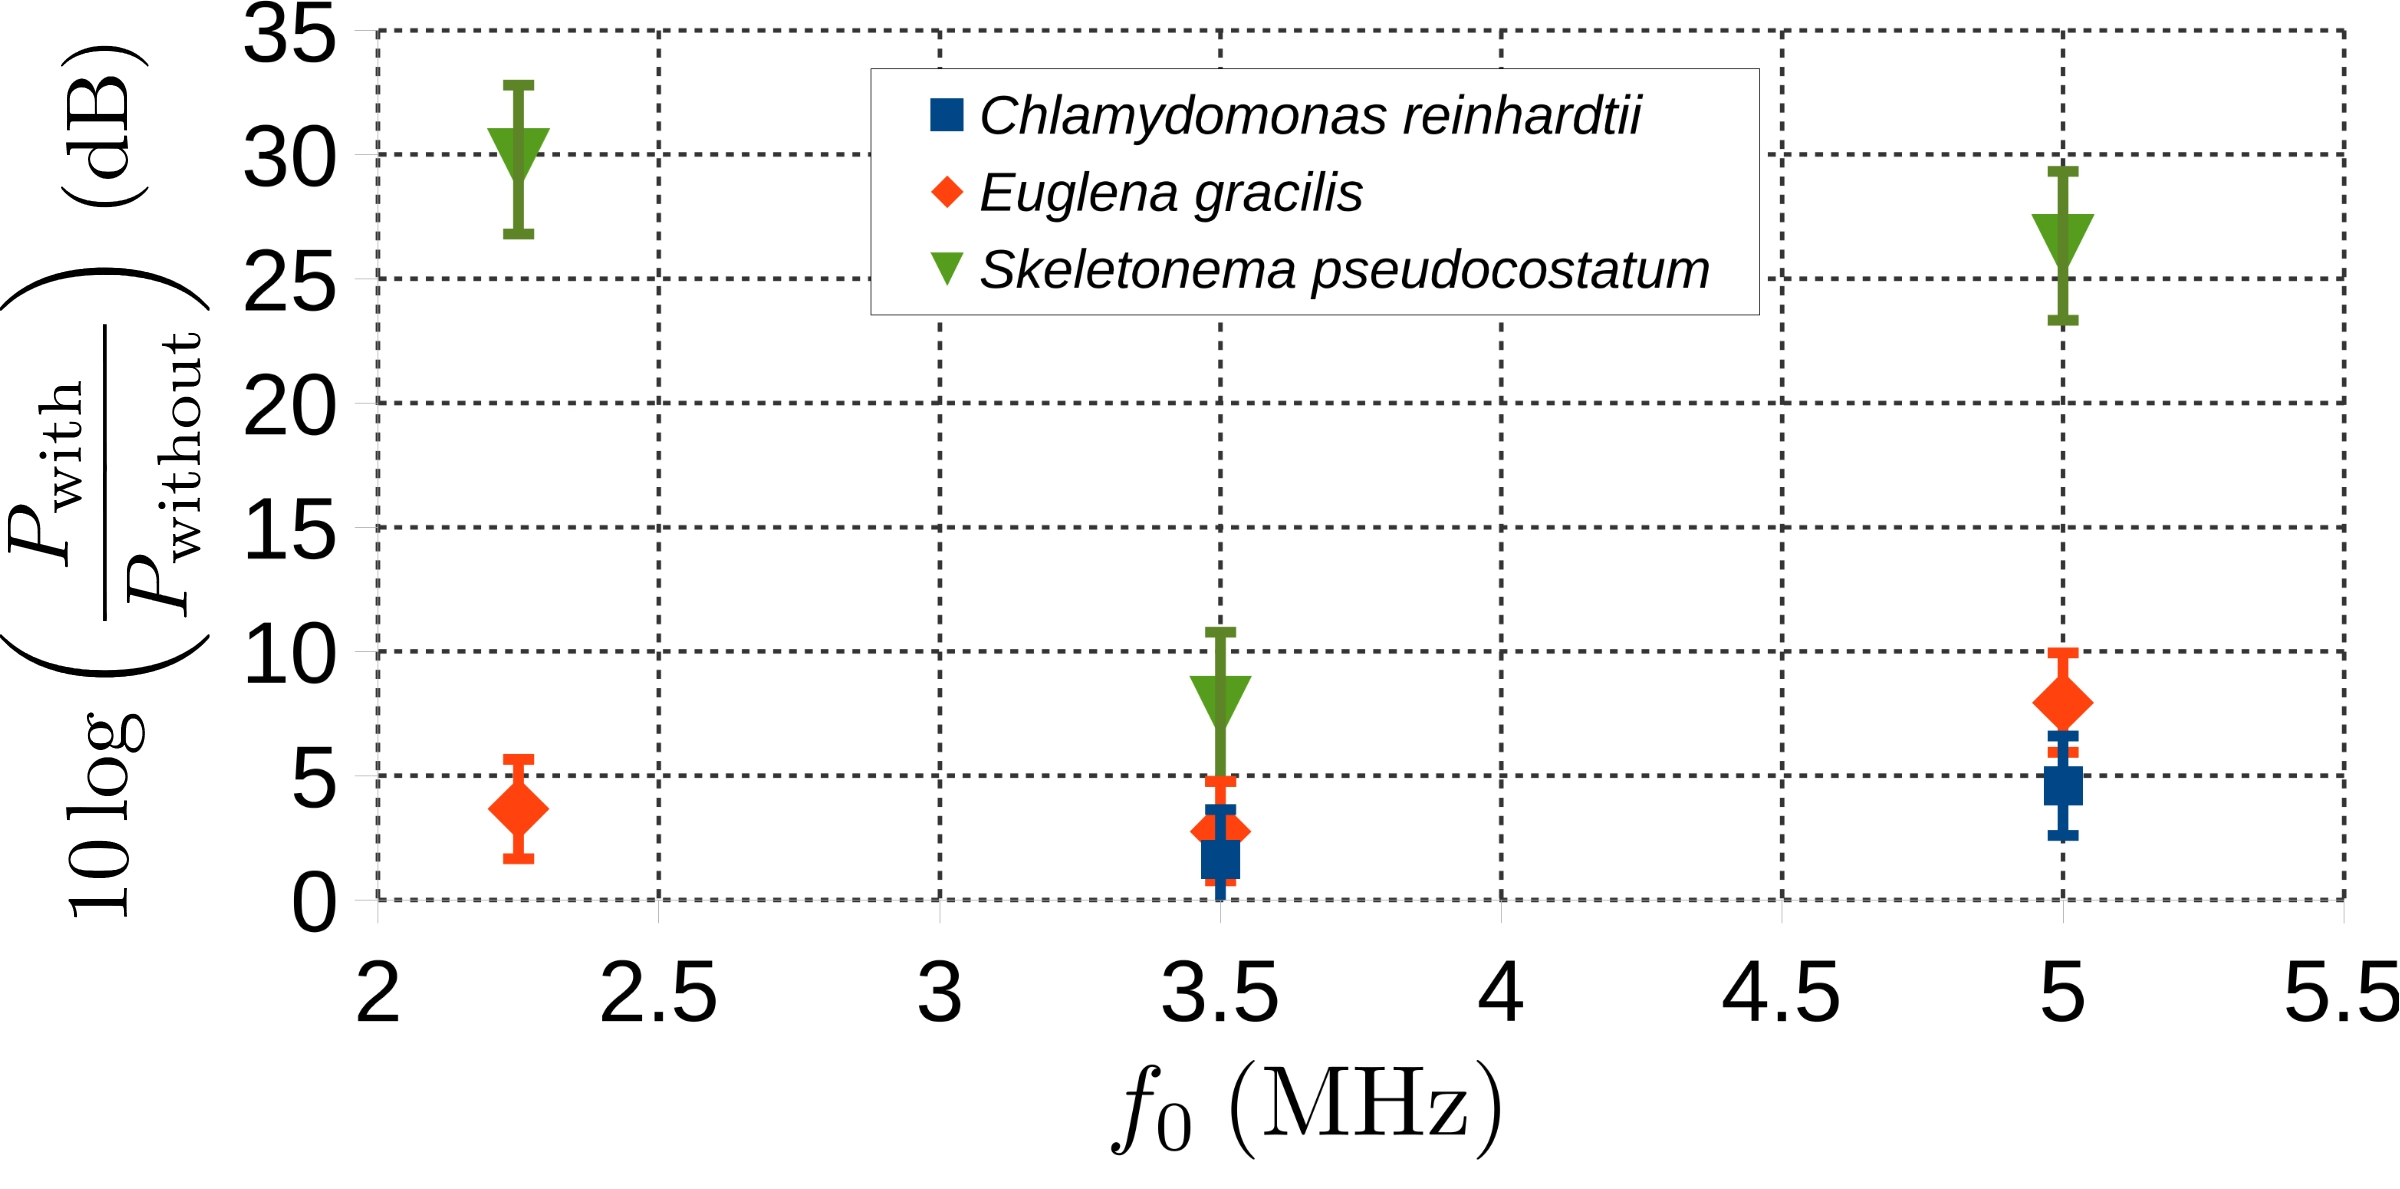
\includegraphics[width=0.6\paperwidth]{imagenes/Ibs_vs_frec22.jpg}}

\begin{itemize}
\item<3-> Higher contrast was observed:
\begin{itemize}
\Fontable
\item<3-> When using 2.25 MHz transducer, due to its higher output acoustic power.
\item<3-> In \textcolor{darkgreen}{{\bf \textit{Skeletonema pseudocostatum}}}, due primarly to their silicon dioxide shell and chain cells arrangements.
\end{itemize}
\end{itemize}

\end{frame}

\subsection{Comparison of $S_v$}

\begin{frame}{RESULTS - Comparison of $S_v$: Optical vs. Acoustical approach}
\Fontable
\begin{itemize}
\item<2-> $S_v$ determination for each culture of \textcolor{darkgreen}{\bf \textit{Skeletonema pseudocostatum}} at 5 MHz, by two methodologies:
\begin{itemize}
\Fontable
\item<3-> Backscattering cross section \textbf{modelling} and \textbf{optical} counting.
\item<4-> Backscattered \textcolor{darkblue}{\bf acoustic} signals acquisition.
\end{itemize}
\end{itemize}

\centering
\visible<5->{\hspace{-1pc} 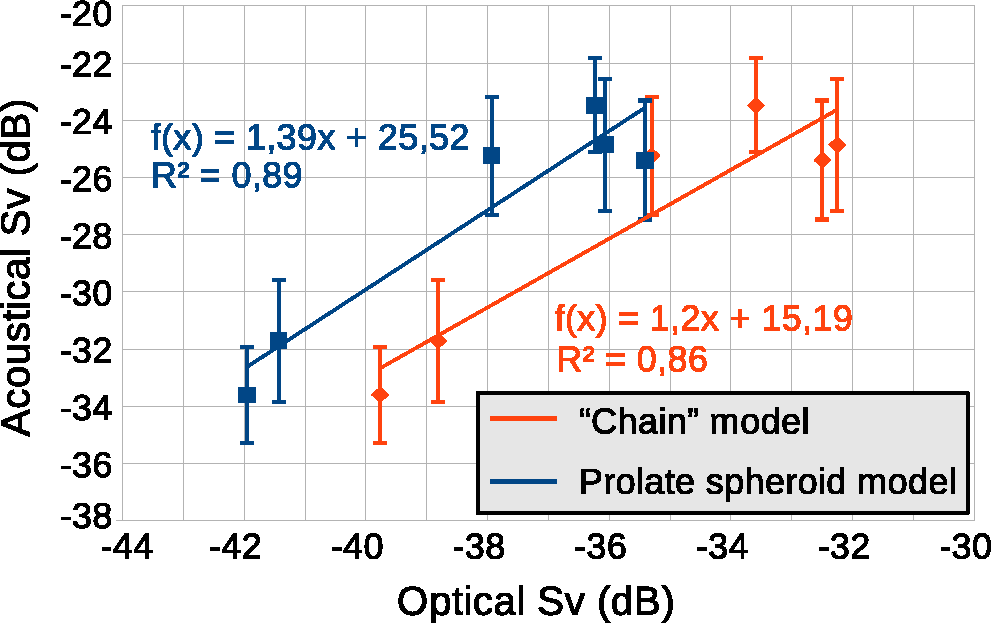
\includegraphics[width=0.6\paperwidth]{imagenes/Svopt_vs_Svac.pdf}}

\end{frame}

\subsection{Simulation of backscattering signals}


\begin{frame}{RESULTS - Simulation of backscattered signals for \textit{Skeletonema} cultures}
\Fontable

\visible<2->{\textcolor{blue}{\textbf{Simulation}} of backscattered signal through the expression:}

\visible<2->{\[
\boxed{\textcolor{blue}{v_\text{sim}(t)=\sum_{k=1}^M \sum_{i=1}^{N_k} A_k \sin(\omega t - t_i) w(t - t_i)}}
\]}

\scriptsize

\only<2-3>{where}

\vspace{0.4pc}

\only<2-3>{$A_k=A_k(\sigma_{\text{bs}_k})$,}

\only<2-3>{$\omega=2\pi f$ is the transducer angular frequency,}

\only<2-3>{$t_i$ is a random number in the selected time interval,}

\only<2-3>{$N_k$ is the numerical abundance of a chain of $k$ elements (individual scatterers),}

\only<2-3>{$w(t)$ is a windowing function with a width given by the emmitted pulse, }

\only<2-3>{M corresponds to the optically observed maximum number of elements per chain.}

\Fontable

\vspace{1pc}
\only<3>{Assumptions:}

\vspace{0.8pc}
\only<3>{$\rightarrow$ All the individual scatterers have the same equivalent radius.}

\only<3>{$\rightarrow$ The number of elements within each chain is \textbf{not necessarily} the same in all the chains.}

\visible<4>{\vspace{-1.9pc} 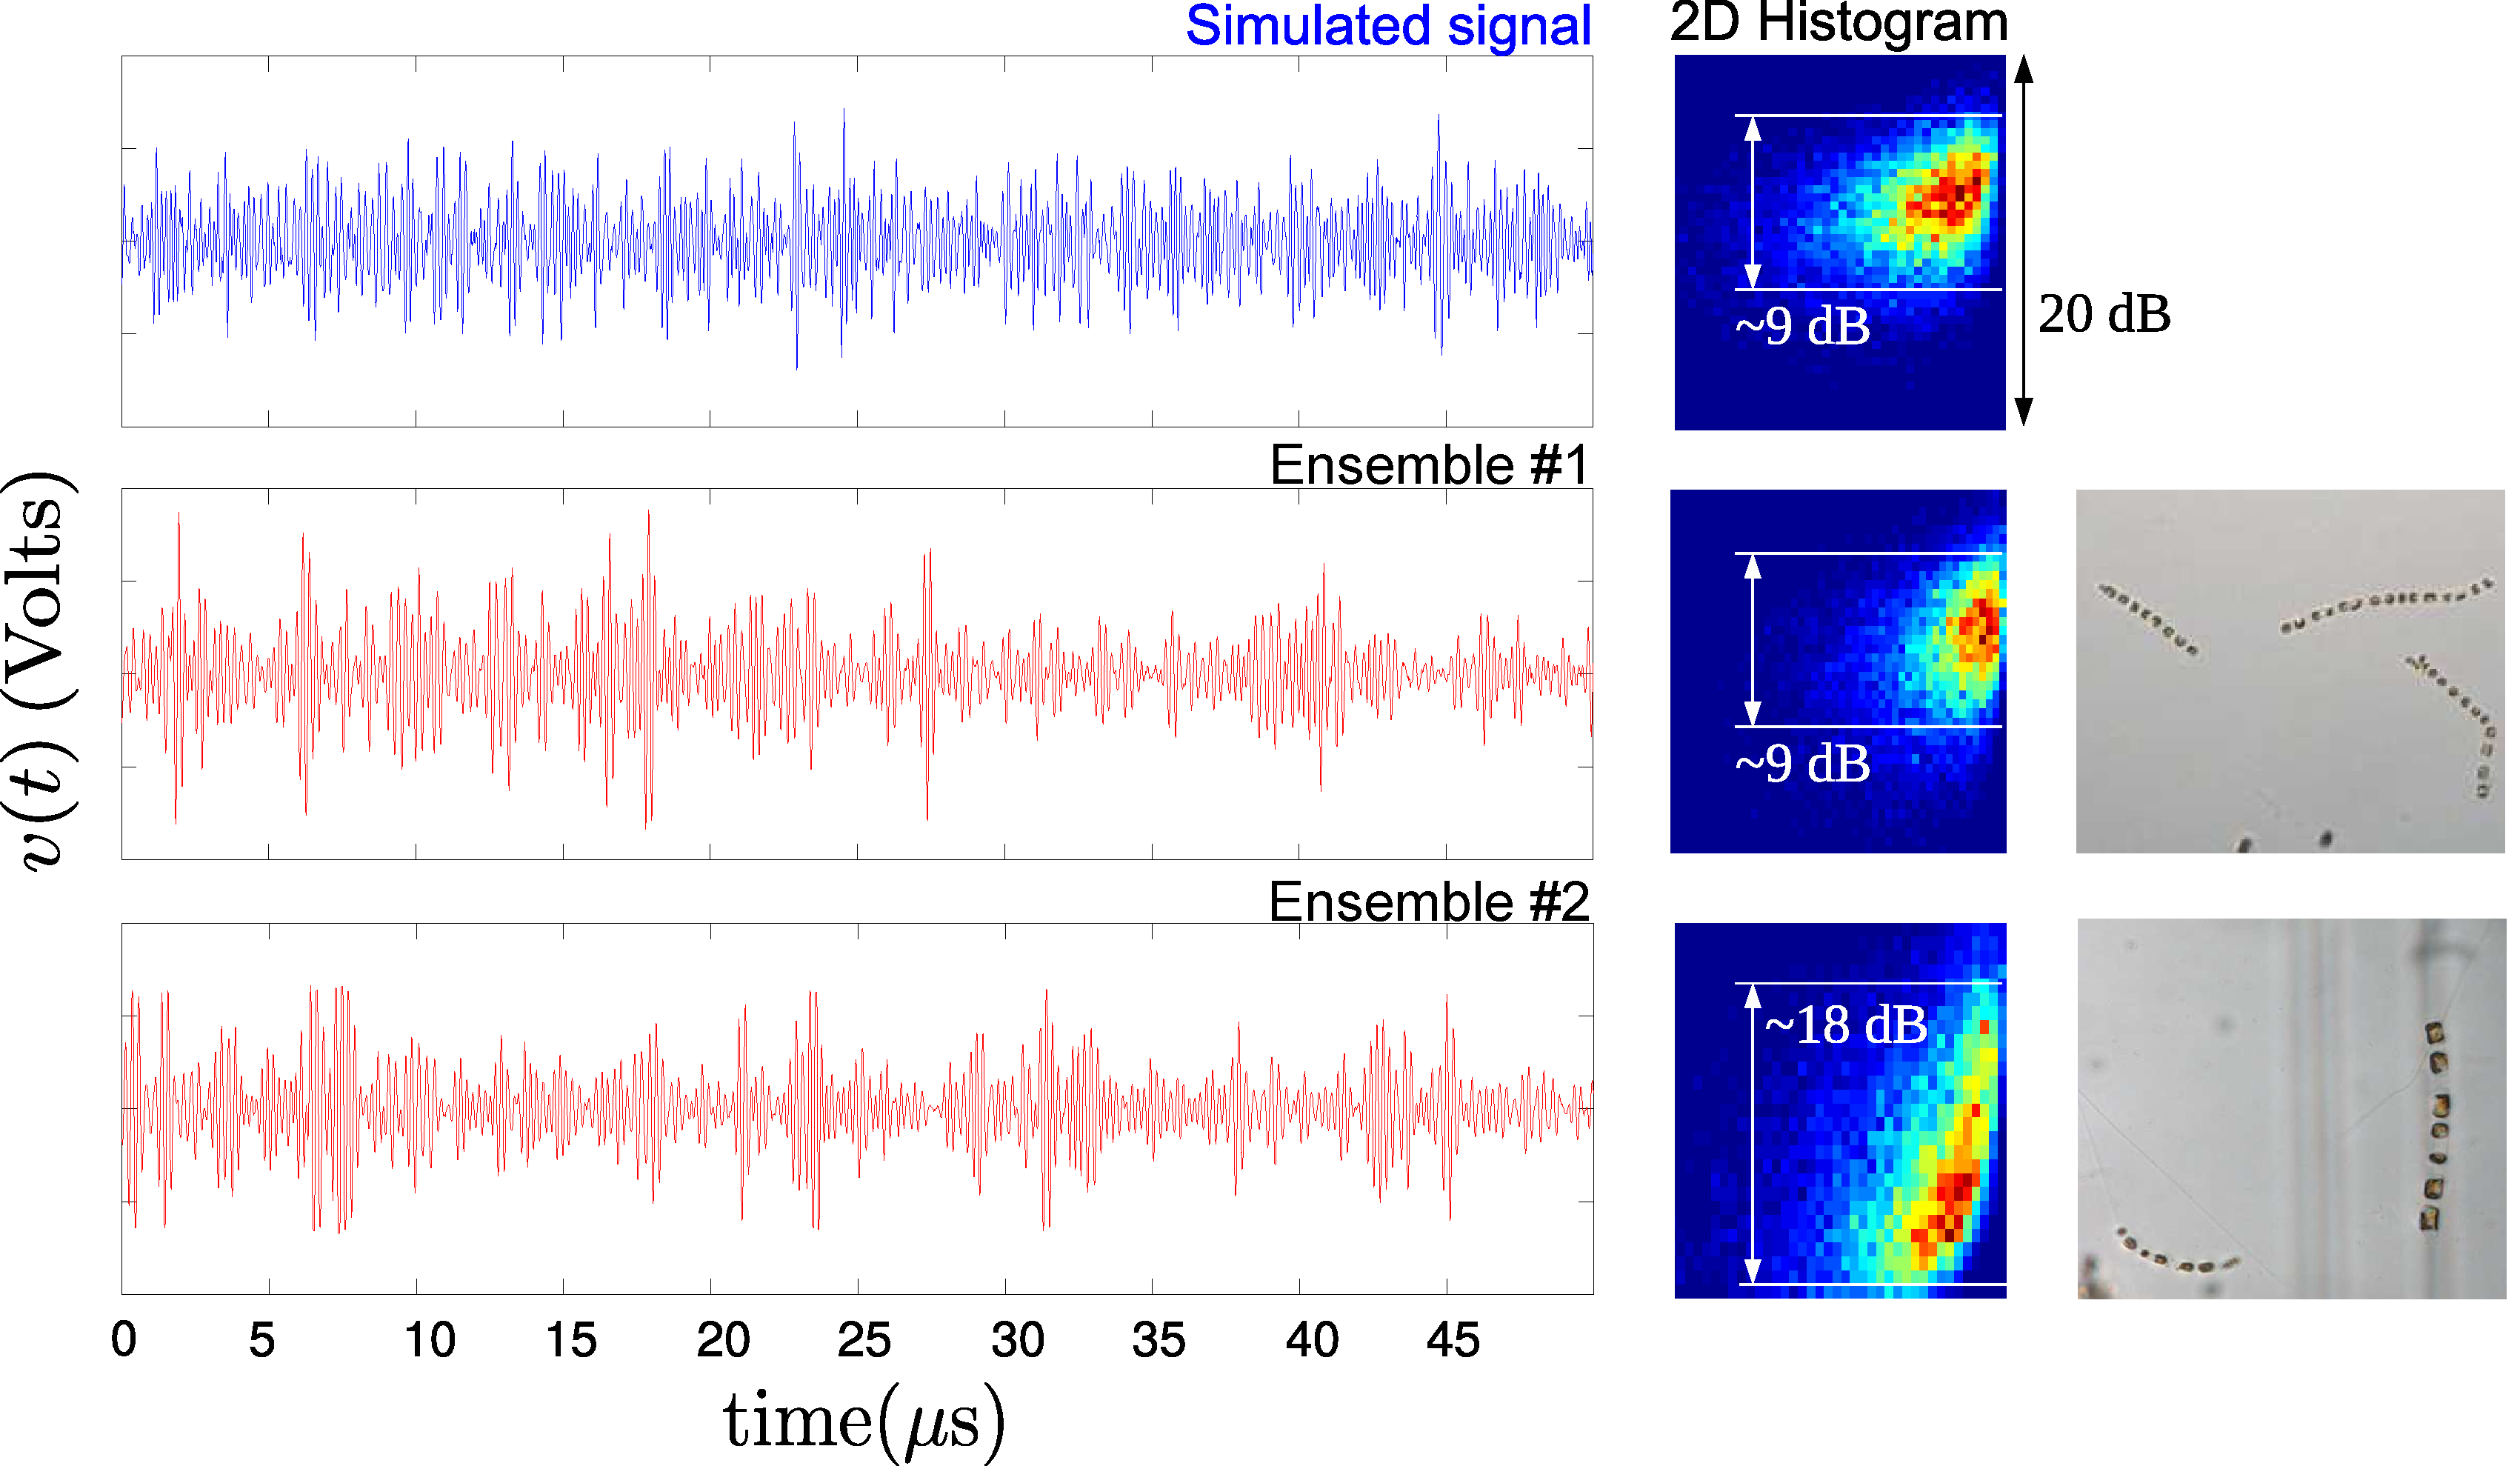
\includegraphics[width=0.75\paperwidth]{imagenes/sim_vs_meas1_okok.pdf}}

\end{frame}

\begin{frame}{RESULTS - Simulation of backscattered signals for \textit{Skeletonema} cultures}
\Fontable

\textcolor{blue}{\textbf{Simulation}} of backscattered signal through the expression:

\[
\boxed{\textcolor{blue}{v_\text{sim}(t)=\sum_{k=1}^M \sum_{i=1}^{N_k} A_k \sin(\omega t - t_i) w(t - t_i)}}
\]

\vspace{5px}
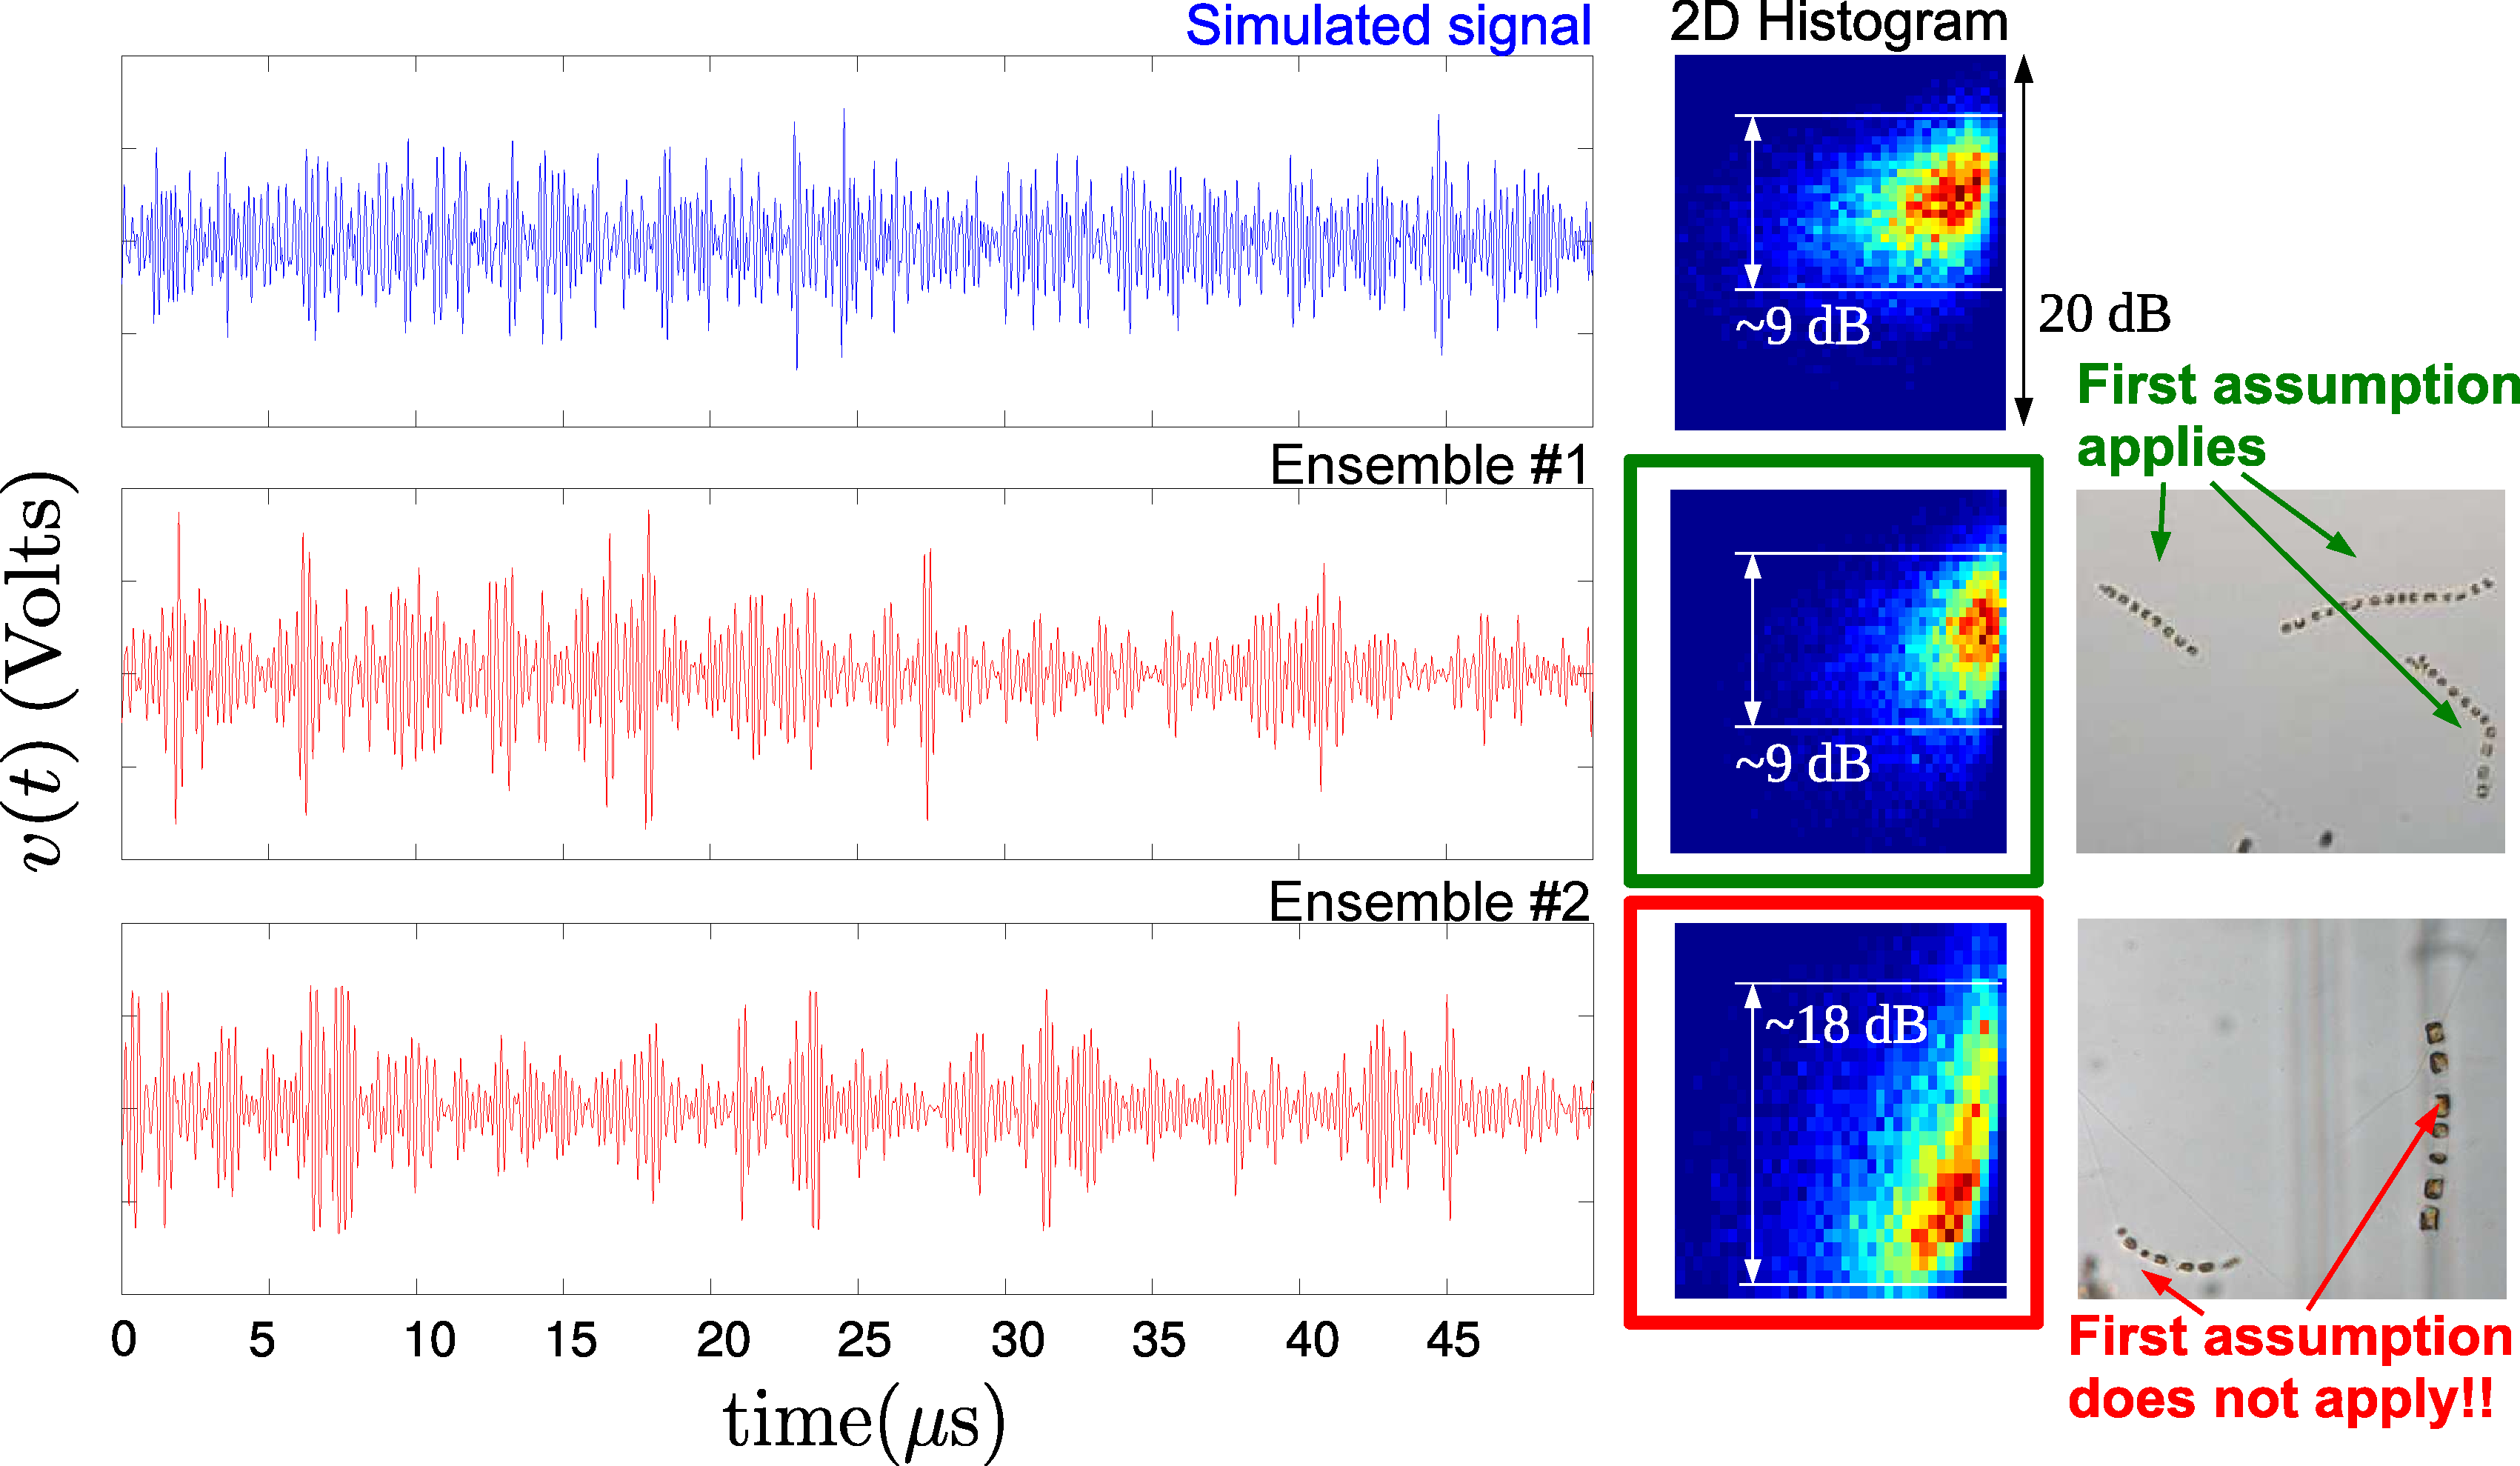
\includegraphics[width=0.75\paperwidth]{imagenes/sim_vs_meas2_okok.pdf}

\end{frame}

\begin{frame}{RESULTS - Simulation of backscattered signals for \textit{Skeletonema} cultures}
\Fontable

\visible<2->{Modification to the original model: two distinct individual scatterers' size: $a_{\text{eq}_2} \gg a_{\text{eq}_1}$ $\Rightarrow$ $\sigma_{\text{bs}_2} \gg \sigma_{\text{bs}_1}$ }

\vspace{0.4pc}
\scriptsize
\visible<2->{where $a_{\text{eq}_i}$ is the equivalent individual scatterer radius.}

\Fontable

\vspace{0.6pc}
\visible<2->{The population characterized by $a_{\text{eq}_i}$ shows:}

\begin{itemize}
\item<2-> Greater backscattering cross section per chain.
\item<2-> Same chain statistical distribution.
\item<2-> Lower number of chains per unit volume.
\end{itemize}

\centering

\vspace{0.6pc}
\only<2>{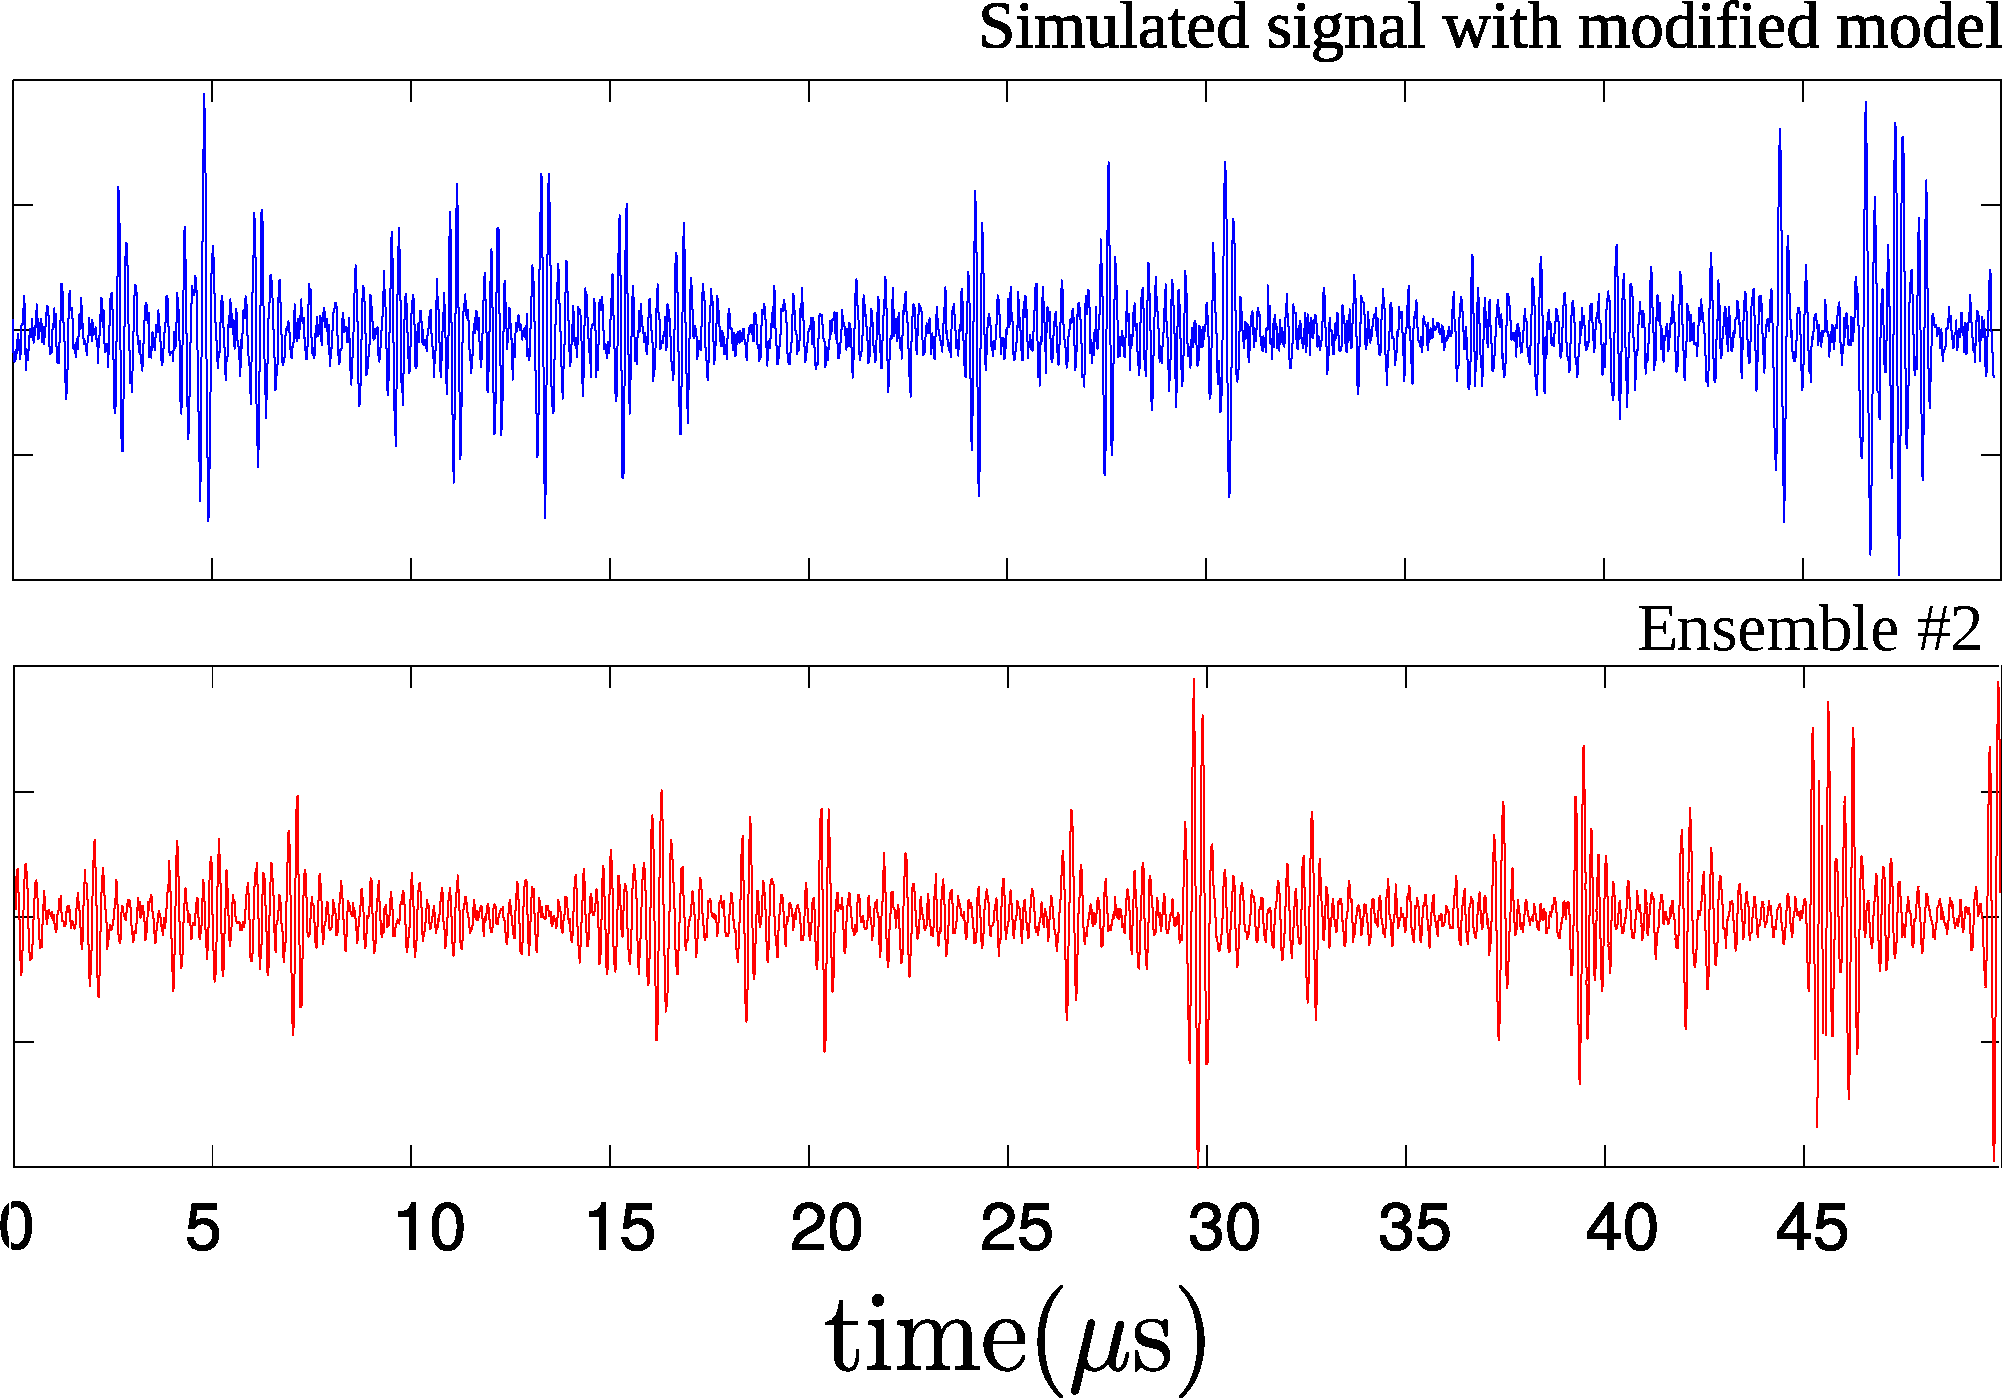
\includegraphics[width=0.48\paperwidth]{imagenes/sim_modif_time_ok.pdf}}
\only<3->{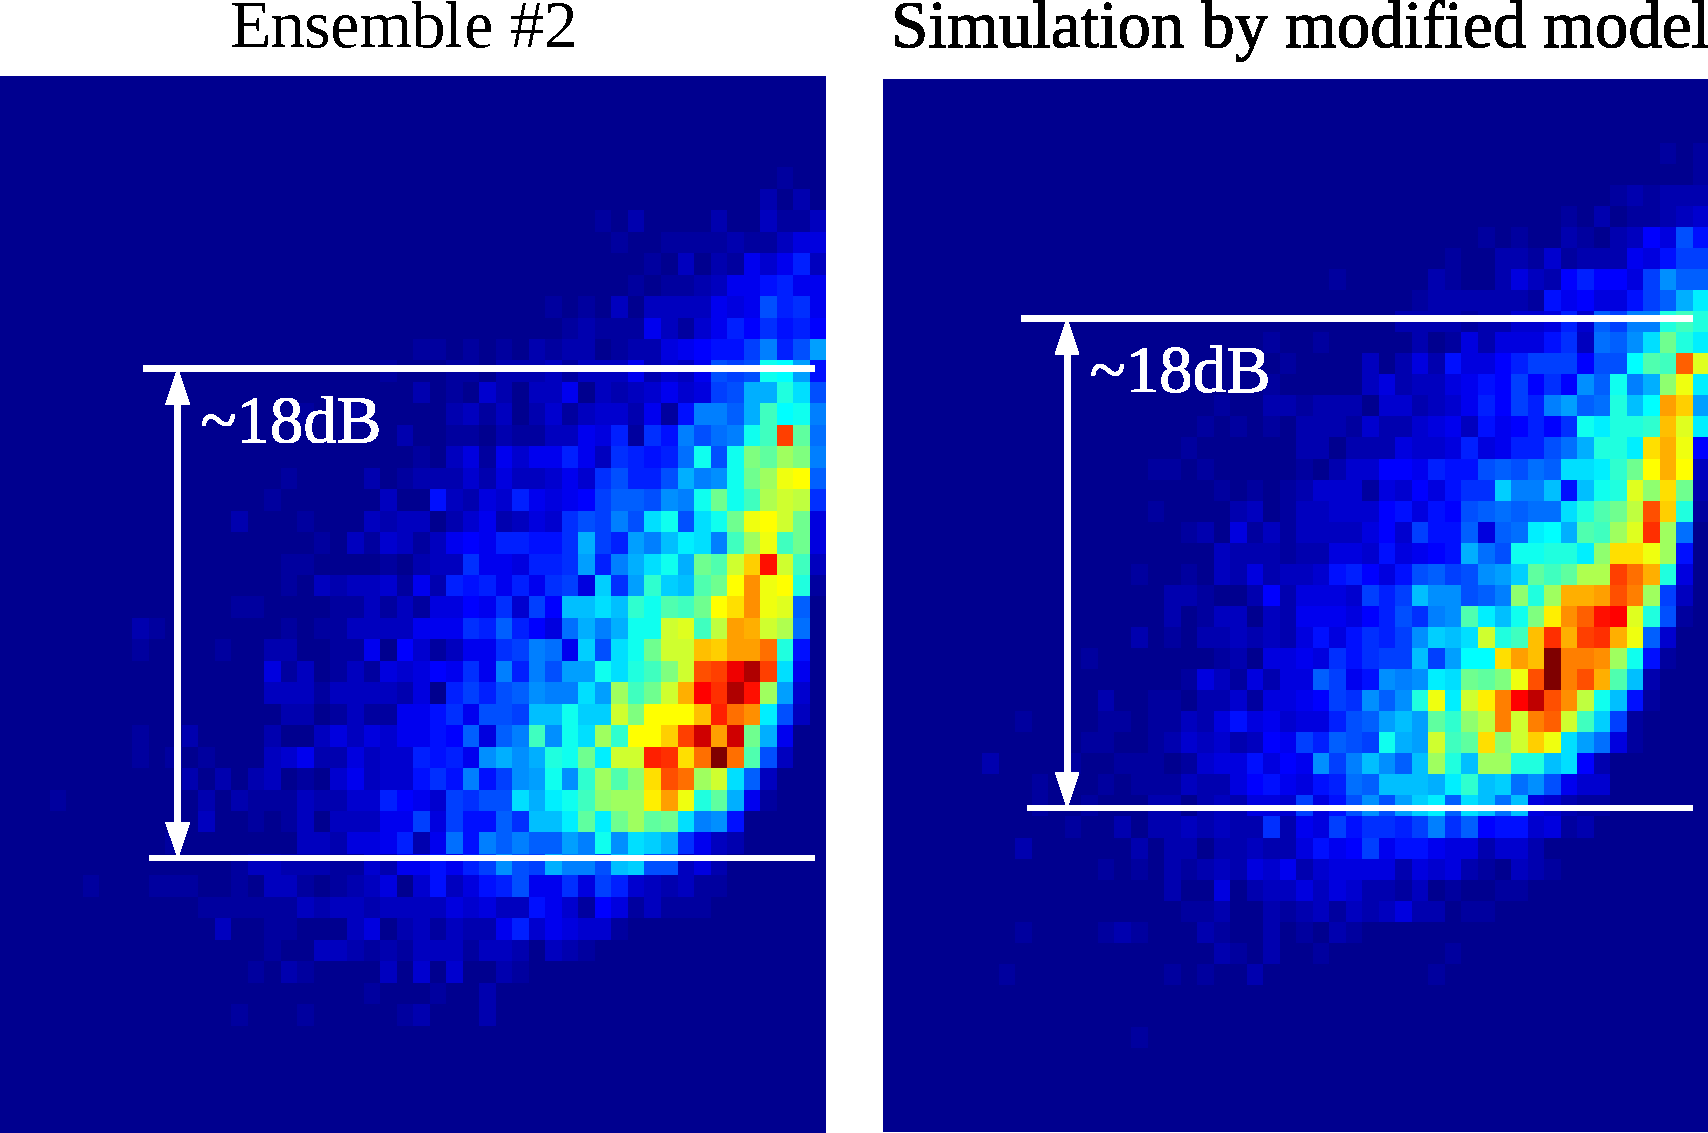
\includegraphics[width=0.49\paperwidth]{imagenes/sim_modif_ok.pdf}}

\end{frame}

\section{Conclusions}

\usebackgroundtemplate{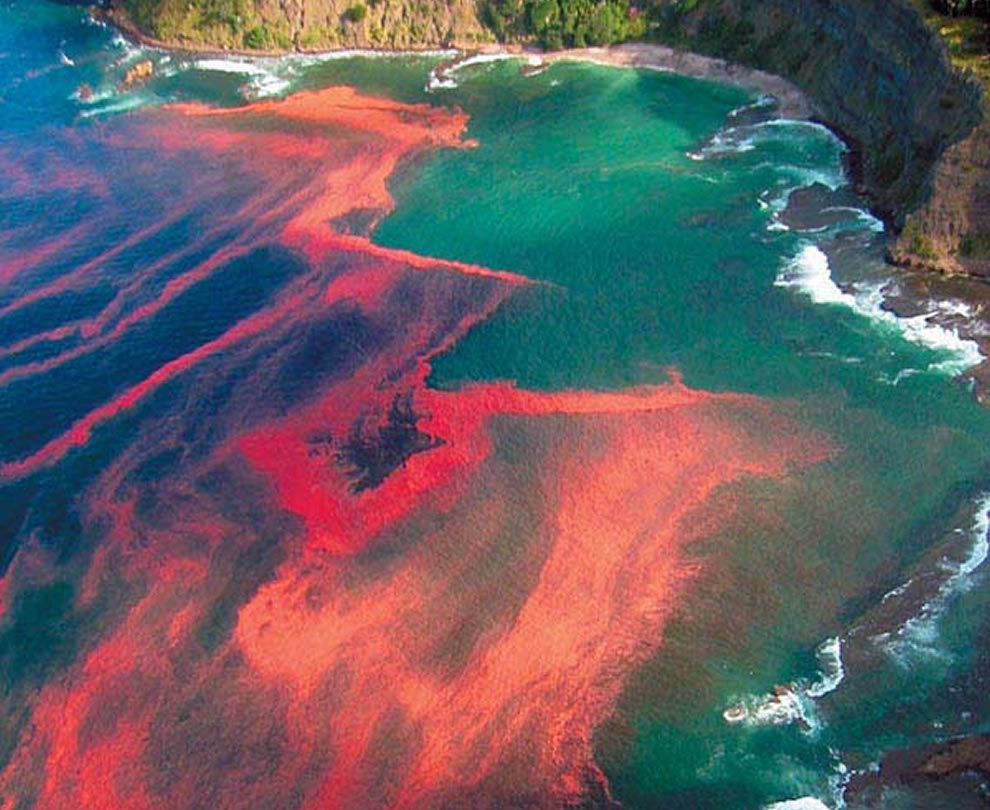
\includegraphics[width=\paperwidth, height=\paperheight]{imagenes/bloom.jpg}}

\begin{frame}{CONCLUSIONS}

\pgfsetfillopacity{0.75}

\visible<2->{

\begin{beamercolorbox}[wd=0.8\paperwidth, ht=0.12\textheight, dp=5px]{block body alerted}
\vfill
\textbf{Acoustic scattering} response was \textbf{detected} for three different \textbf{phytoplanktonic species} at 2.25, 3.5 and 5 MHz.

\end{beamercolorbox}
}

\vspace{0.6pc}
\visible<3->{
\begin{beamercolorbox}[fill, dp=5px]{block body alerted}
\vfill
\textbf{Sensitivity} analysis of the proposed acoustic methodology with respect to \textbf{Numerical Abundance} of \textbf{\textit{Skeletonema}} cultures was carried out.
\end{beamercolorbox}
}

\vspace{0.6pc}
\visible<4->{
\begin{beamercolorbox}[fill, dp=5px]{block body alerted}
\vfill
\textbf{Signal processing} techniques were applied to \textbf{minimize} spurious scatterers contribution, \textbf{improving} acoustic determination of backscattered power.
\end{beamercolorbox}
}

\vspace{0.6pc}
\visible<5->{
\begin{beamercolorbox}[fill, dp=5px]{block body alerted}
\vfill
Simulations of backscattered signal led to validate the used backscattering cross section models.
\end{beamercolorbox}
}

\vspace{0.6pc}
\visible<6->{
\begin{beamercolorbox}[fill, dp=5px]{block body alerted}
\vfill
Current results \textbf{encourage} further work on \textbf{acoustic detection} of Harmful Algae Blooms.
\end{beamercolorbox}
}

\end{frame}

\usebackgroundtemplate{}

\newgeometry{margin=0.5cm}
\begin{frame}[plain,t]
\vspace{0.4cm}

\centering
\Huge
\textcolor{darkblue}{\textbf{MANY THANKS!}}

\Large
\textcolor{darkblue}{\textbf{Questions?}}

\vspace{0.6pc}

\normalsize

\begin{flushleft}
\hspace{0.3cm}
\textcolor{black}{\textbf{The authors:}}
\end{flushleft}

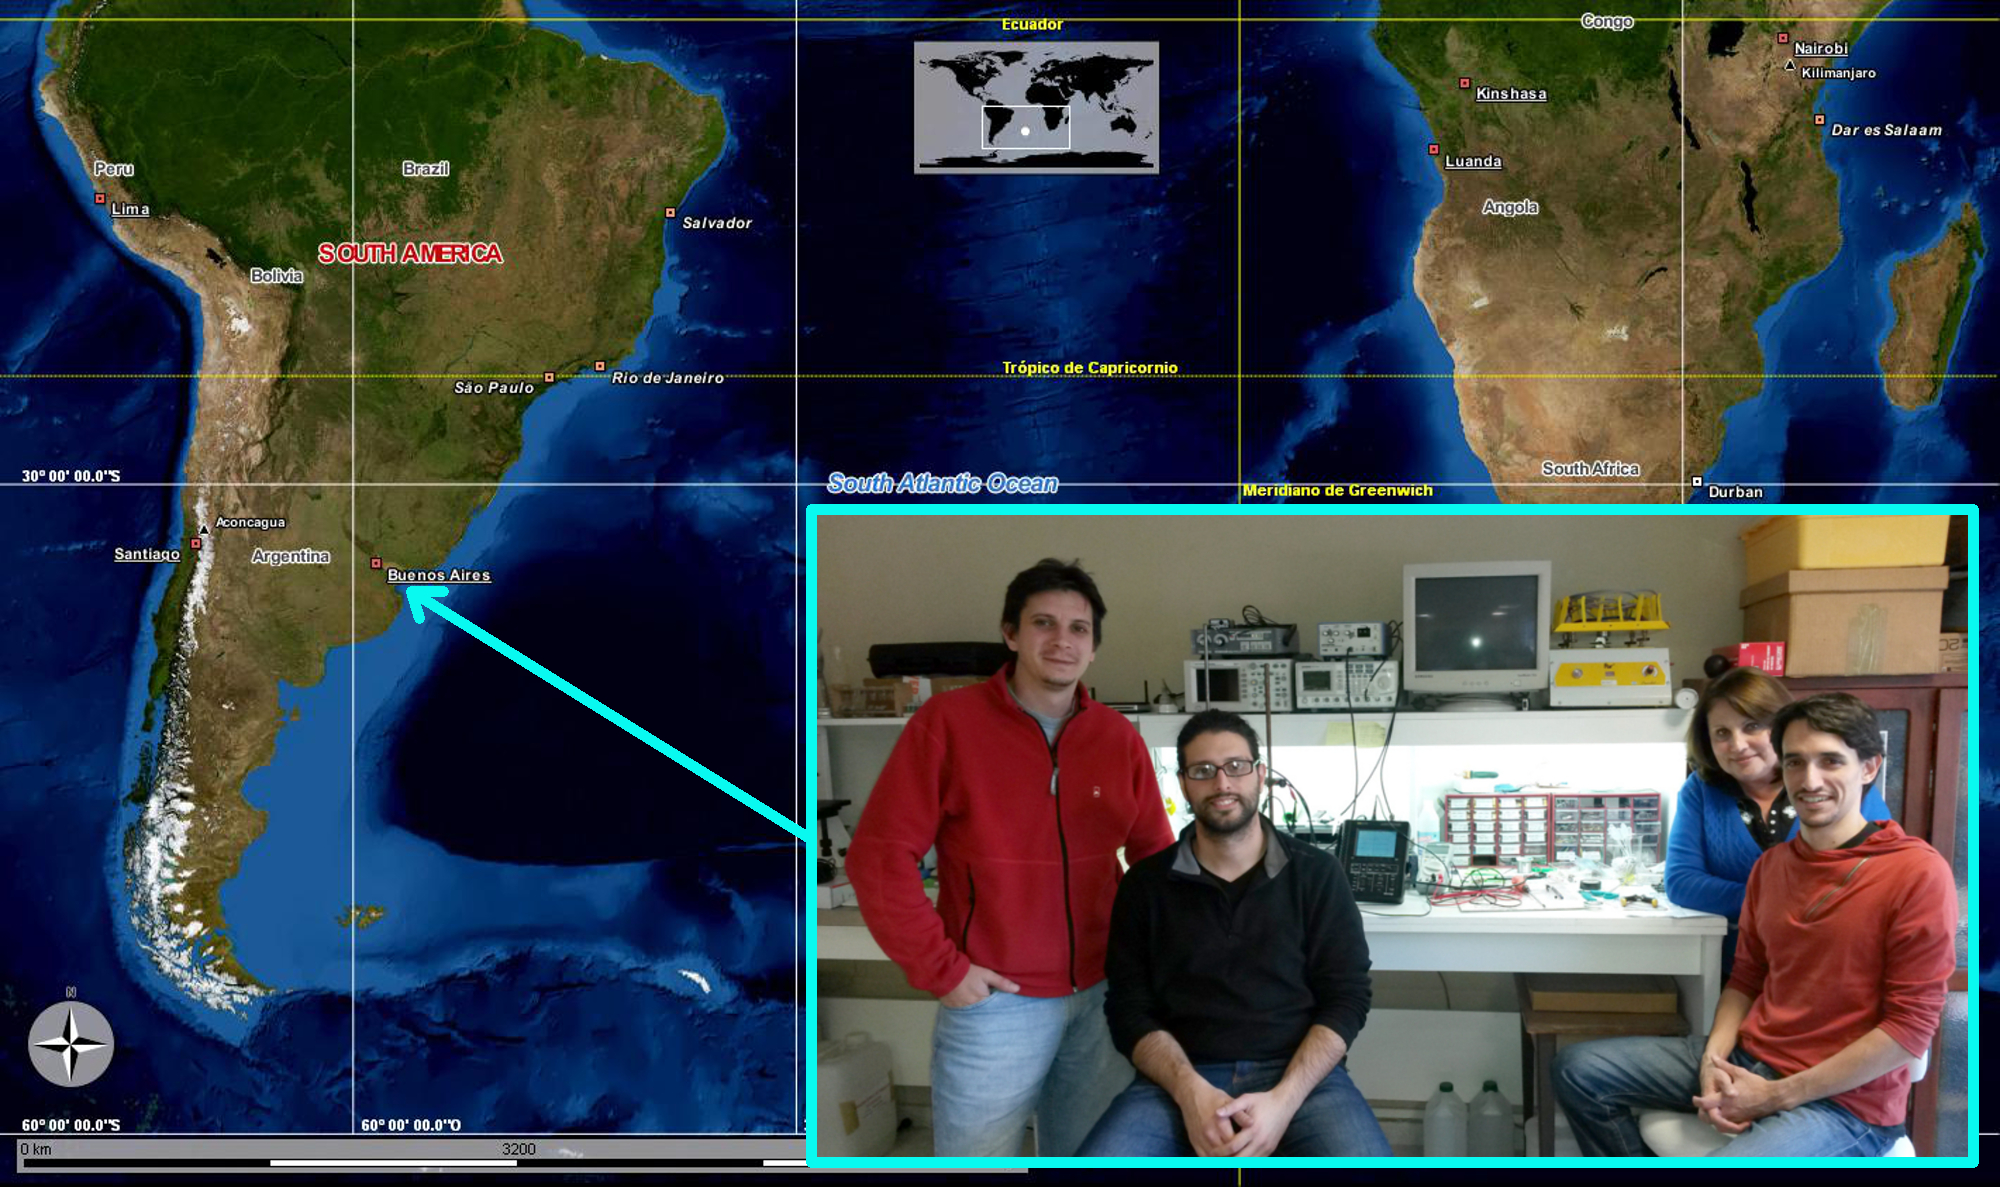
\includegraphics[width=0.85\paperwidth]{imagenes/Argentina_FitoAcusticos.jpg}

\end{frame}

%\begingroup
%\makeatletter
%\setlength{\hoffset}{-.5\beamer@sidebarwidth}
%\makeatother
%\begin{frame}[plain]
%
%\centering
%\Huge
%MANY THANKS!
%\normalsize
%
%The authors:
%
%
%\begin{flushleft}
%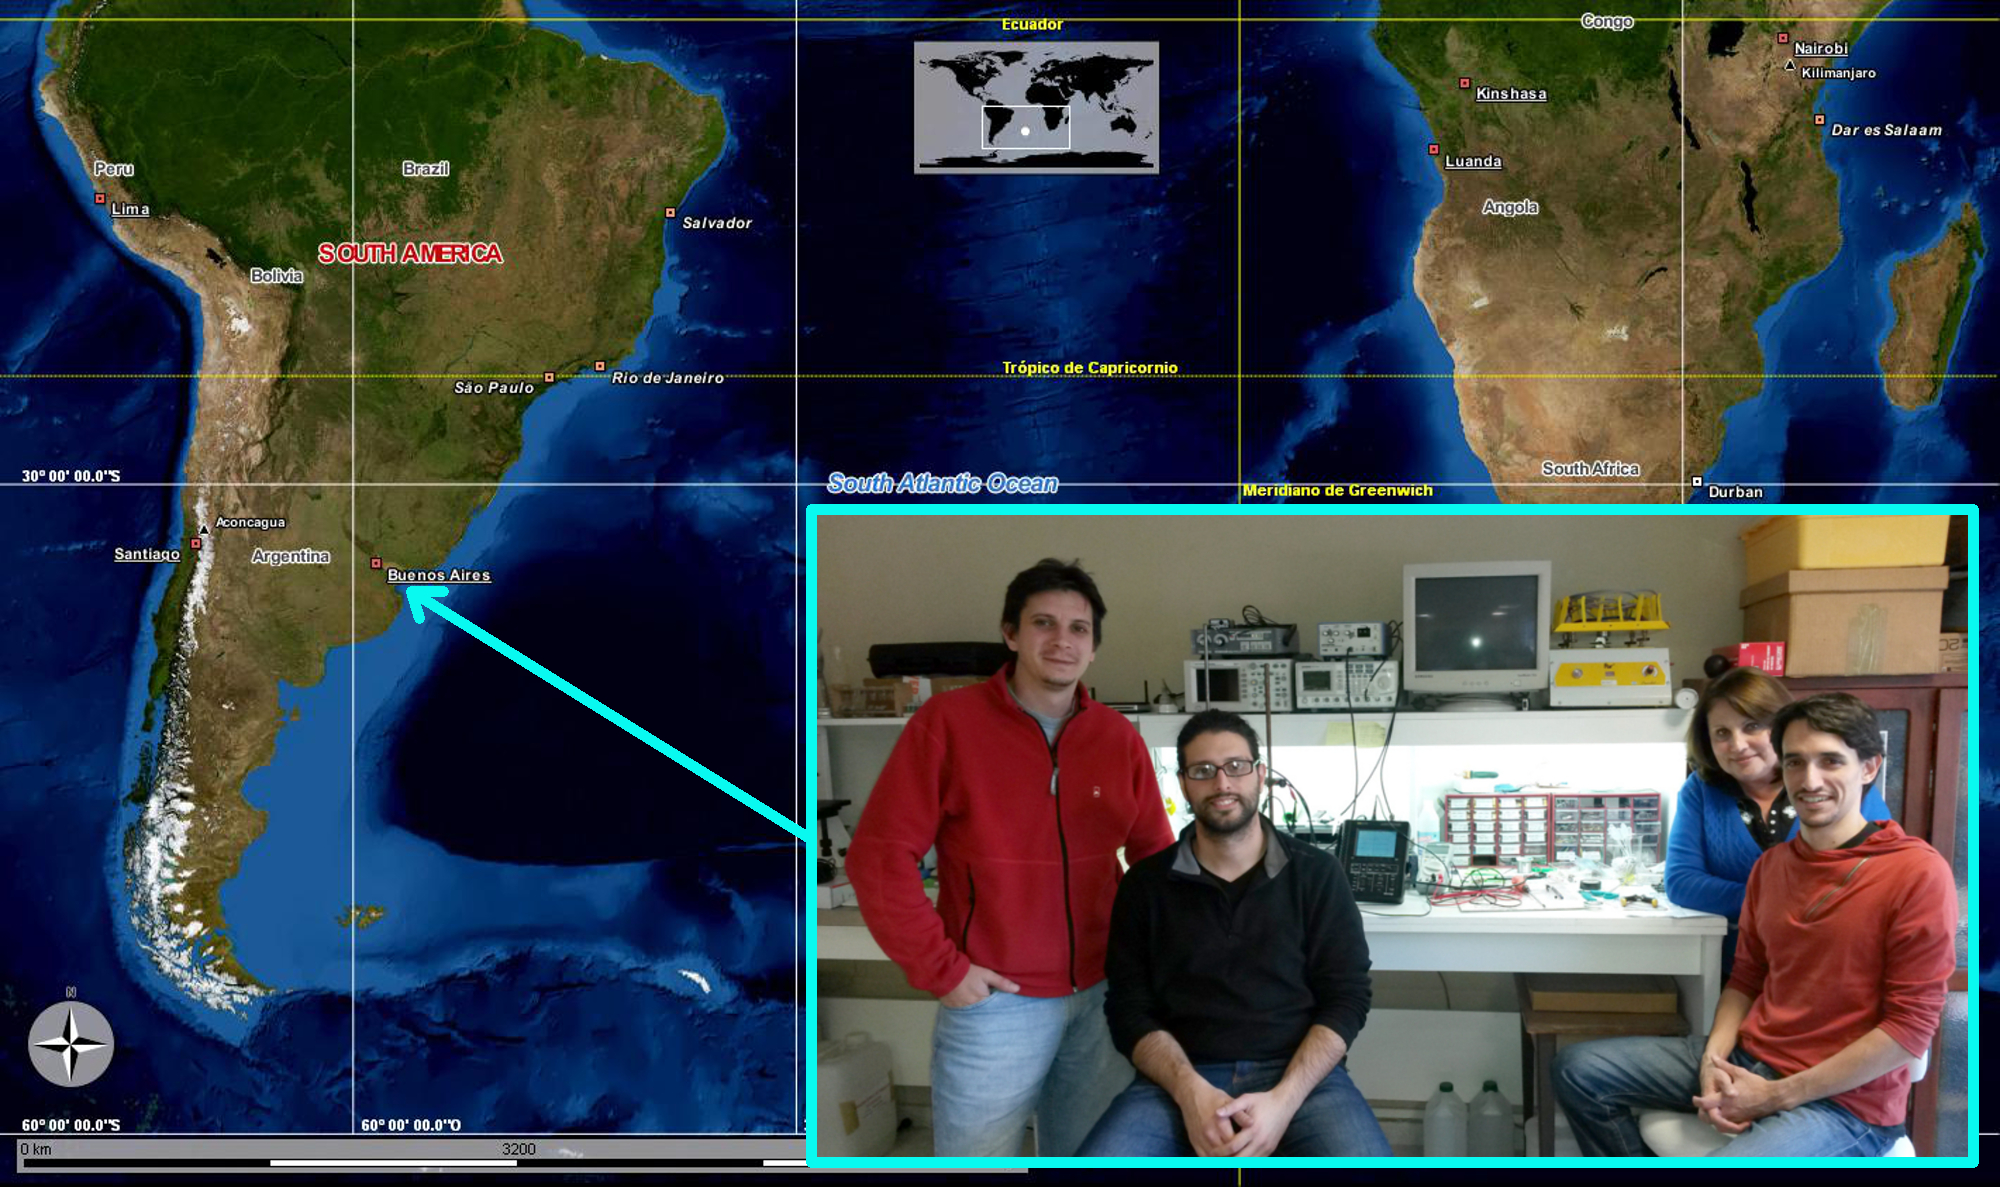
\includegraphics[width=0.9\paperwidth]{imagenes/Argentina_FitoAcusticos.jpg}
%\end{flushleft}
%
%\end{frame}
%\endgroup


\end{document}


